\documentclass[UTF8,a4paper,zihao=-4]{ctexart}

\usepackage[left=2.6cm,right=2.4cm,top=2.5cm,bottom=2.5cm]{geometry}
\usepackage{amsmath,amssymb,bm}
\usepackage{booktabs,longtable,tabularx,array,multirow}
\usepackage{graphicx,float,caption}
\usepackage{xcolor}
\usepackage{fancyhdr}
\usepackage{setspace}
\usepackage{enumitem}
\usepackage{listings}
\usepackage{placeins}
\usepackage{hyperref}

\setmainfont{Times New Roman}
\setmonofont{Cascadia Mono}
\setCJKmainfont[AutoFakeBold=2]{SimSun}
\setCJKsansfont{Microsoft YaHei}
\setlength{\parindent}{2em}
\setlength{\parskip}{0pt}
\linespread{1.28}
\setlist{nosep,leftmargin=2.2em}
\captionsetup{font=small,labelsep=quad}
\graphicspath{{../figures/question1/png/}{../figures/question2/png/}{../figures/question3/png/}{../figures/question4/png/}}

\pagestyle{fancy}
\fancyhf{}
\fancyfoot[C]{\thepage}
\renewcommand{\headrulewidth}{0pt}

\ctexset{
  section={format=\bfseries\zihao{4},beforeskip=1.1ex,afterskip=0.6ex},
  subsection={format=\bfseries\zihao{-4},beforeskip=0.8ex,afterskip=0.4ex},
  subsubsection={format=\bfseries\zihao{-4},beforeskip=0.6ex,afterskip=0.3ex}
}

\hypersetup{colorlinks=true,linkcolor=black,citecolor=black,urlcolor=blue,pdfauthor={},pdftitle={基于稳健时序外推与可信域多目标优化的锂离子电池快充策略研究}}

\definecolor{codegray}{RGB}{245,245,245}
\definecolor{codegreen}{RGB}{0,105,62}
\lstset{
  language=Python,
  basicstyle=\ttfamily\tiny,
  keywordstyle=\color{blue!70!black},
  commentstyle=\color{codegreen},
  stringstyle=\color{red!55!black},
  backgroundcolor=\color{codegray},
  numbers=left,
  numberstyle=\tiny\color{gray},
  stepnumber=1,
  numbersep=6pt,
  frame=single,
  breaklines=true,
  breakatwhitespace=false,
  showstringspaces=false,
  columns=fullflexible,
  keepspaces=true,
  tabsize=4,
  inputencoding=utf8,
  extendedchars=true
}

\newcommand{\SOH}{\mathrm{SOH}}
\newcommand{\EOL}{\mathrm{EOL}}
\newcommand{\dd}{\mathrm{d}}
\newcommand{\R}{\mathbb{R}}
\newcommand{\secref}[1]{第\ref{#1}节}

\begin{document}

\begin{center}
  {\bfseries\zihao{2} 基于稳健时序外推与可信域多目标优化的\\[0.35em]锂离子电池快充策略研究}
\end{center}

\vspace{0.8em}
\noindent{\bfseries 摘要：}
针对两阶段恒流快充条件下磷酸铁锂电池的退化表征、寿命估计、测试电池预测与策略优化问题，本文建立了“稳健清洗—时间截断验证—群体与个体融合—可信域 Pareto 优化”的统一框架。首先保留全部原始记录，仅对 3 个孤立物理异常点作局部修复，并用稳健 LOWESS 重建 SOH 曲线；以局部 Theil--Sen 估计提取节点 SOH、分窗斜率、曲率及温度、内阻、充电时间等辅助特征。对 40 块训练电池按时间顺序进行 100/150 次截断验证，比较线性、受约束二次、幂律和指数模型，最终选择单调受约束二次模型。其 150 次截断预测 151--200 次的中位 MAE 为 $3.12\times10^{-4}$，估计寿命中位数为 1348.7 次，但模型结构敏感性表明该寿命只能解释为 SOH 达到 0.8 的条件性外推指标。

其次，以电池为基本观测单位，用 Welch、Kruskal--Wallis、置换检验、效应量和分组 bootstrap 研究策略及参数关系。策略对 SOH$_{200}$、50--200 次退化率和估计寿命的置换检验 $p$ 值分别为 0.01955、0.00015 和 0.00815；S8 的早期退化最明显。较高 $C_2$ 与更差早期指标存在趋势，但批次控制后明显减弱，故不作因果解释。对 9 块测试电池，构造留一电池的同策略模板、个体残差修正、监督岭回归及自适应集成。40 块训练电池严格伪测试中，集成模型的平均 MAE、RMSE 分别为 $2.77\times10^{-4}$、$3.61\times10^{-4}$，较最优单模型的 RMSE 降低 8.2\%，并输出测试电池逐循环区间与条件性 EOL。

最后在 NEWSTRUCTURE 同批次的 6 个策略上，以两阶段理想时间加经验偏移建立充电时间模型，以 SOC 加权应力建立单调退化代理，并仅在观测凸包与局部信任域交集内搜索。得到 413 个非支配候选；推荐的稳健区域约为 $C_1,C_2=4.8\sim4.9\,\mathrm C$、$Q_1=55\%\sim60\%$。knee 代表点 $(4.85\mathrm C,55\%,4.85\mathrm C)$ 的预测时间为 10.121 min、SOH$_{200}$ 为 0.9957、条件性 EOL 为 1472 次。所有优化点均是待实验验证的模型候选，而非已证实的最优策略。

\vspace{0.6em}
\noindent{\bfseries 关键词：}锂离子电池；快速充电；SOH 退化；时间截断验证；集成预测；Pareto 优化

\newpage

\section{问题重述与研究思路}\label{sec:intro}

题目给出 49 块 A123 18650 磷酸铁锂电池在两阶段恒流快充下的早期循环数据，其中 40 块非测试电池记录至第 200 次循环，9 块测试电池仅公开至第 150 次循环。已有研究表明，早期循环信号可用于寿命预测与快充策略筛选\cite{severson2019,attia2020}，但本题缺少真实完整寿命标签，必须额外约束外推结论的可信边界。充电策略记为
\[
  x=(C_1,Q_1,C_2),
\]
表示先以倍率 $C_1$ 充至荷电状态 $Q_1$，再以倍率 $C_2$ 充至 80\% SOC。循环寿命统一定义为预测 SOH 首次不高于 0.8 时的循环次数，而附件不含完整真实寿命标签。因此本文所称 EOL 是依据早期退化曲线得到的条件性指标，不等同于实测失效时刻。

四问存在明显的递进关系：问题一决定清洗口径、早期表征和统一寿命指标；问题二在不虚增样本量的前提下分析策略整体与参数的统计关系；问题三模拟真实的“前 150 次预测后 50 次”场景并预测 9 块测试电池；问题四在批次可比、参数邻域可信的范围内寻找充电时间与退化的非支配解。为防止后续模型互相矛盾，问题二至四均复用问题一的稳健 SOH，不再重新清洗。

本文的核心原则是：所有预测验证保持时间顺序；所有群体信息在伪测试中按电池留一；循环级数据不被当成相互独立的大样本；已观测的短期预测性能、EOL 的长期结构不确定性和优化点的实验外推风险分开报告。

\section{模型假设与符号说明}\label{sec:assumption}

作如下必要假设：同一电池循环序号可作为退化时间轴；经局部异常修复后的短时 SOH 波动主要为测量与工况扰动，稳健平滑不改变总体退化方向；在第 200 次循环以后仅作单调、低复杂度外推；同一 strategy 内电池可共享群体趋势，但允许个体偏移、斜率和轻度曲率不同；连续优化仅在已有参数点的凸包及局部邻域内有效。温度、内阻和充电时间仅作关联性辅助变量，不据此宣称独立因果效应。

\begin{table}[H]
\centering
\caption{主要符号}
\begin{tabularx}{0.94\textwidth}{>{\centering\arraybackslash}p{2.2cm}X}
\toprule
符号 & 含义 \\
\midrule
$i,t,p$ & 电池编号、循环次数、充电策略编号 \\
$y_i(t)$ & 电池 $i$ 在循环 $t$ 的稳健 SOH \\
$C_1,Q_1,C_2$ & 第一阶段倍率、切换 SOC、第二阶段倍率 \\
$D_i$ & 第 50--200 次循环的稳健 SOH 衰减量，取 $-100\hat\beta_{50:200}$ \\
$\widehat L_i$ & 受约束退化模型首次达到 $\SOH=0.8$ 的循环次数 \\
$\mu_p(t)$ & 留一规则下策略 $p$ 的群体平均 SOH 模板 \\
$S_p(x)$ & 指数为 $p$ 的 SOC 加权充电应力 \\
$T(x)$ & 从 0\% SOC 充至 80\% SOC 的预测时间 \\
$\mathcal H,\mathcal N$ & 观测参数凸包、局部最近邻信任域 \\
\bottomrule
\end{tabularx}
\end{table}

\section{数据清洗与早期退化表征}\label{sec:data}

\subsection{完整性检查与保守清洗}

汇总表含 49 行、13 列，电池编号唯一；循环表含 9350 行、9 列，$(battery\_id,cycle)$ 无重复且关键字段无缺失。40 块非测试电池覆盖 1--200 次，9 块测试电池覆盖 1--150 次。逐字段检查容量、SOH、内阻、温度和充电时间后，只发现 3 个孤立明显异常：B1 第 12 次容量与 SOH 尖峰，以及 B2、B3 第 12 次内阻为 0。本文不删除整行，而用同一电池相邻循环的稳健局部估计替代相应单元格，原值与修复值同时保存在异常记录表中。

不直接采用附件的 \texttt{SOH\_smooth}。先以 Hampel 型局部中位数与 MAD 识别孤立偏离，再对清理后的原始 SOH 使用鲁棒 LOWESS\cite{cleveland1979}：局部拟合迭代降低大残差权重，平滑跨度约 25 个循环。图\ref{fig:q1clean}表明处理只修正尖峰而没有改变真实下降趋势。

\begin{figure}[H]
\centering
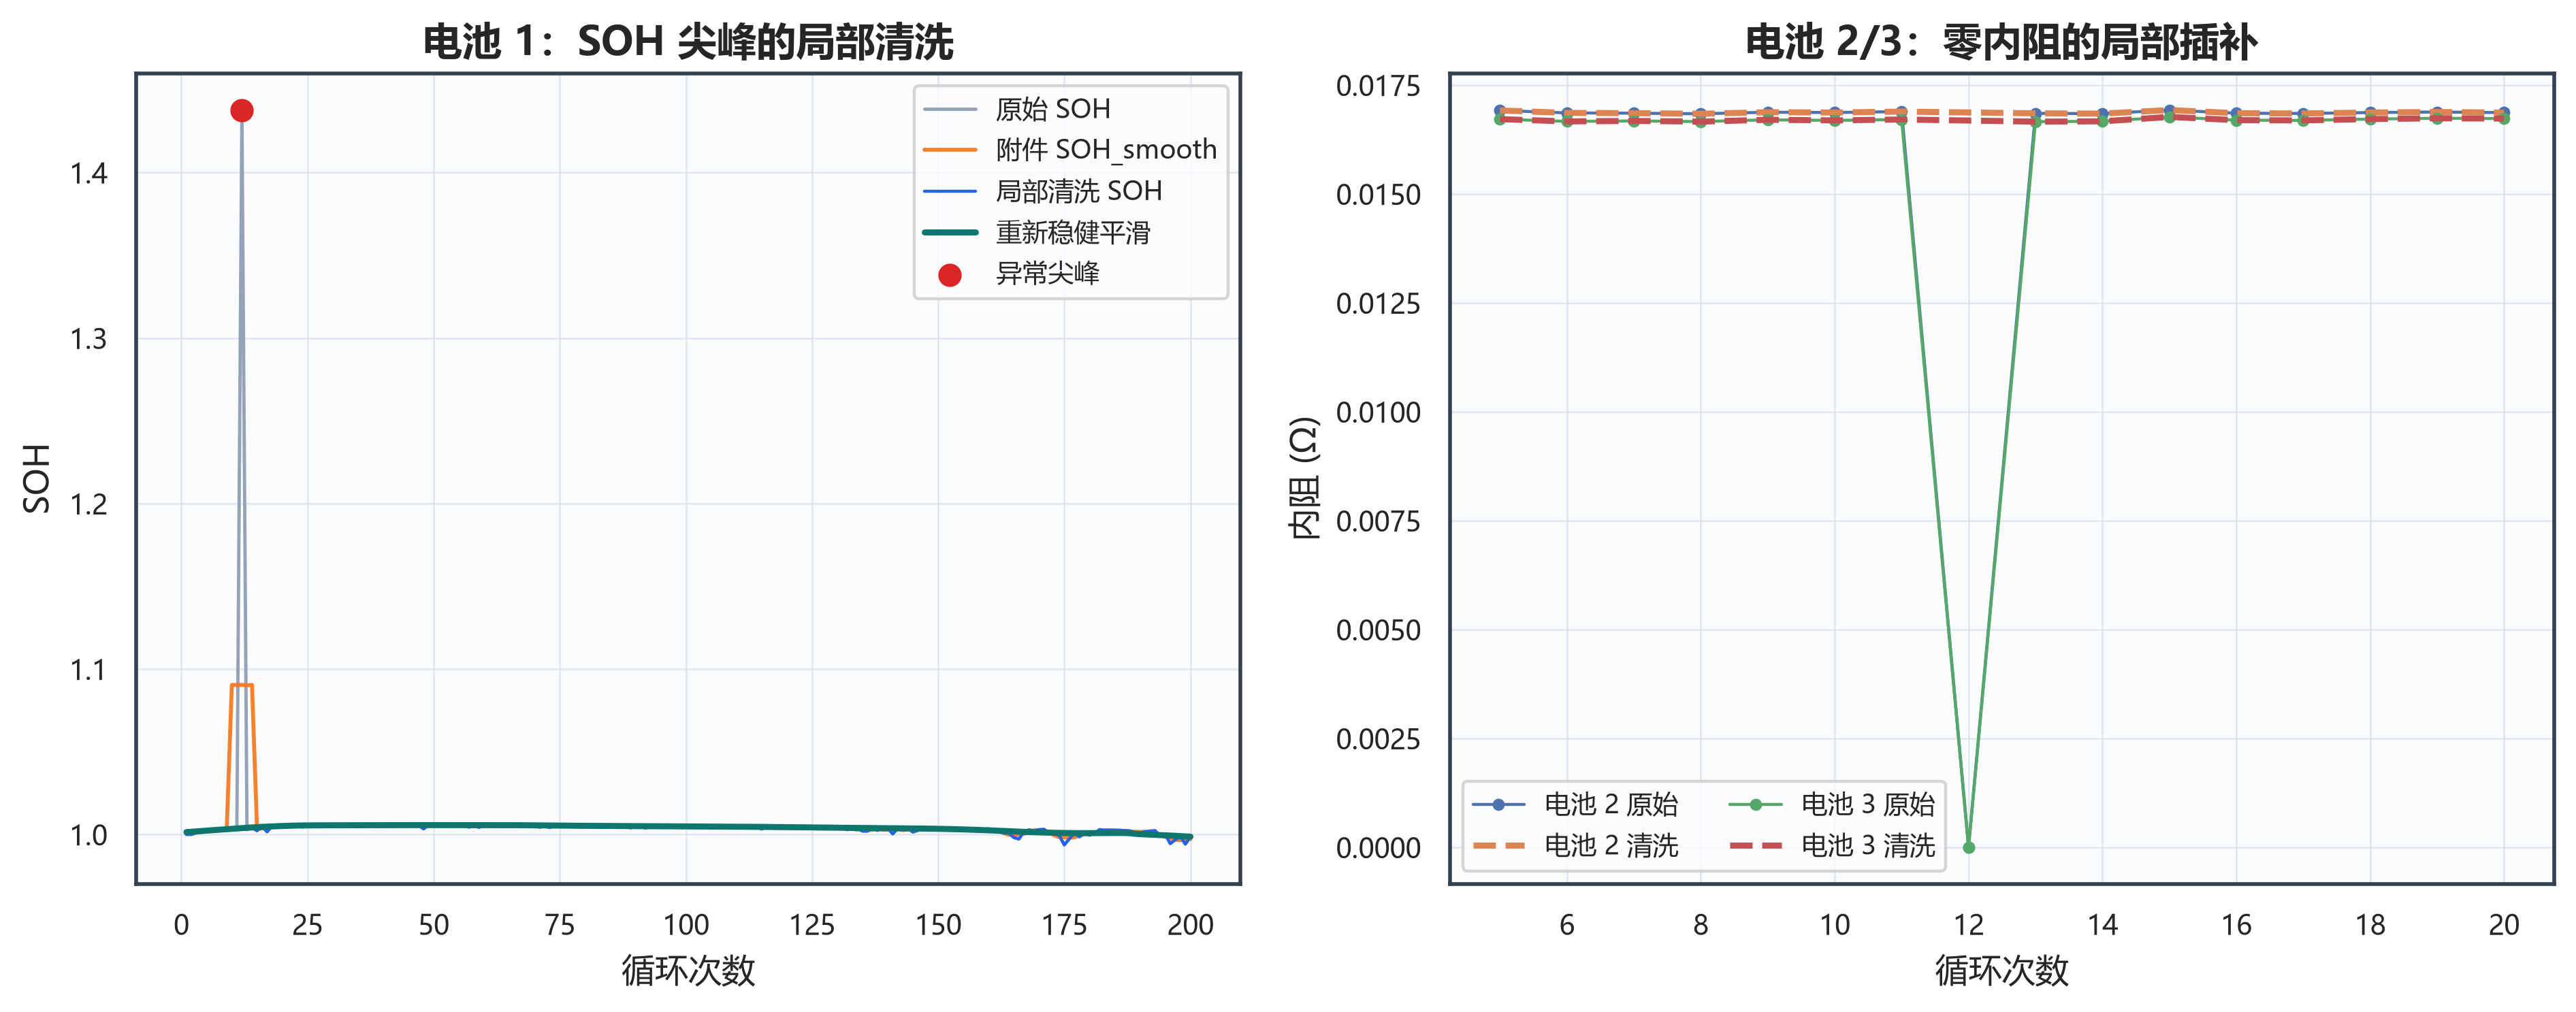
\includegraphics[width=0.92\textwidth]{q1_04_cleaning_before_after.png}
\caption{典型异常电池清洗前后对比}
\label{fig:q1clean}
\end{figure}

\subsection{稳健早期特征}

对节点 $t_0\in\{50,100,150,200\}$，在邻域内用 Theil--Sen 直线\cite{sen1968}估计 $y_i(t_0)$；对 $[1,50]$、$[50,100]$、$[100,150]$、$[150,200]$ 和 $[50,200]$ 分别估计每 100 次循环的稳健斜率。定义
\[
  D_i=-100\widehat\beta_{i,50:200},\qquad
  A_i=100\left(\widehat\beta_{i,150:200}-\widehat\beta_{i,50:100}\right),
\]
并以 LOWESS 残差的 MAD 表示短时波动。温度、内阻、充电时间均提取均值和随循环的稳健趋势，作为后续偏离诊断的辅助特征。

整体 SOH 曲线及策略分组见图\ref{fig:q1all}。S4--S7 与 S9 在 200 次内下降较慢，而 S8 早期下降最明显；该图只反映观察性差异，不能单独识别倍率的独立作用。

\begin{figure}[H]
\centering
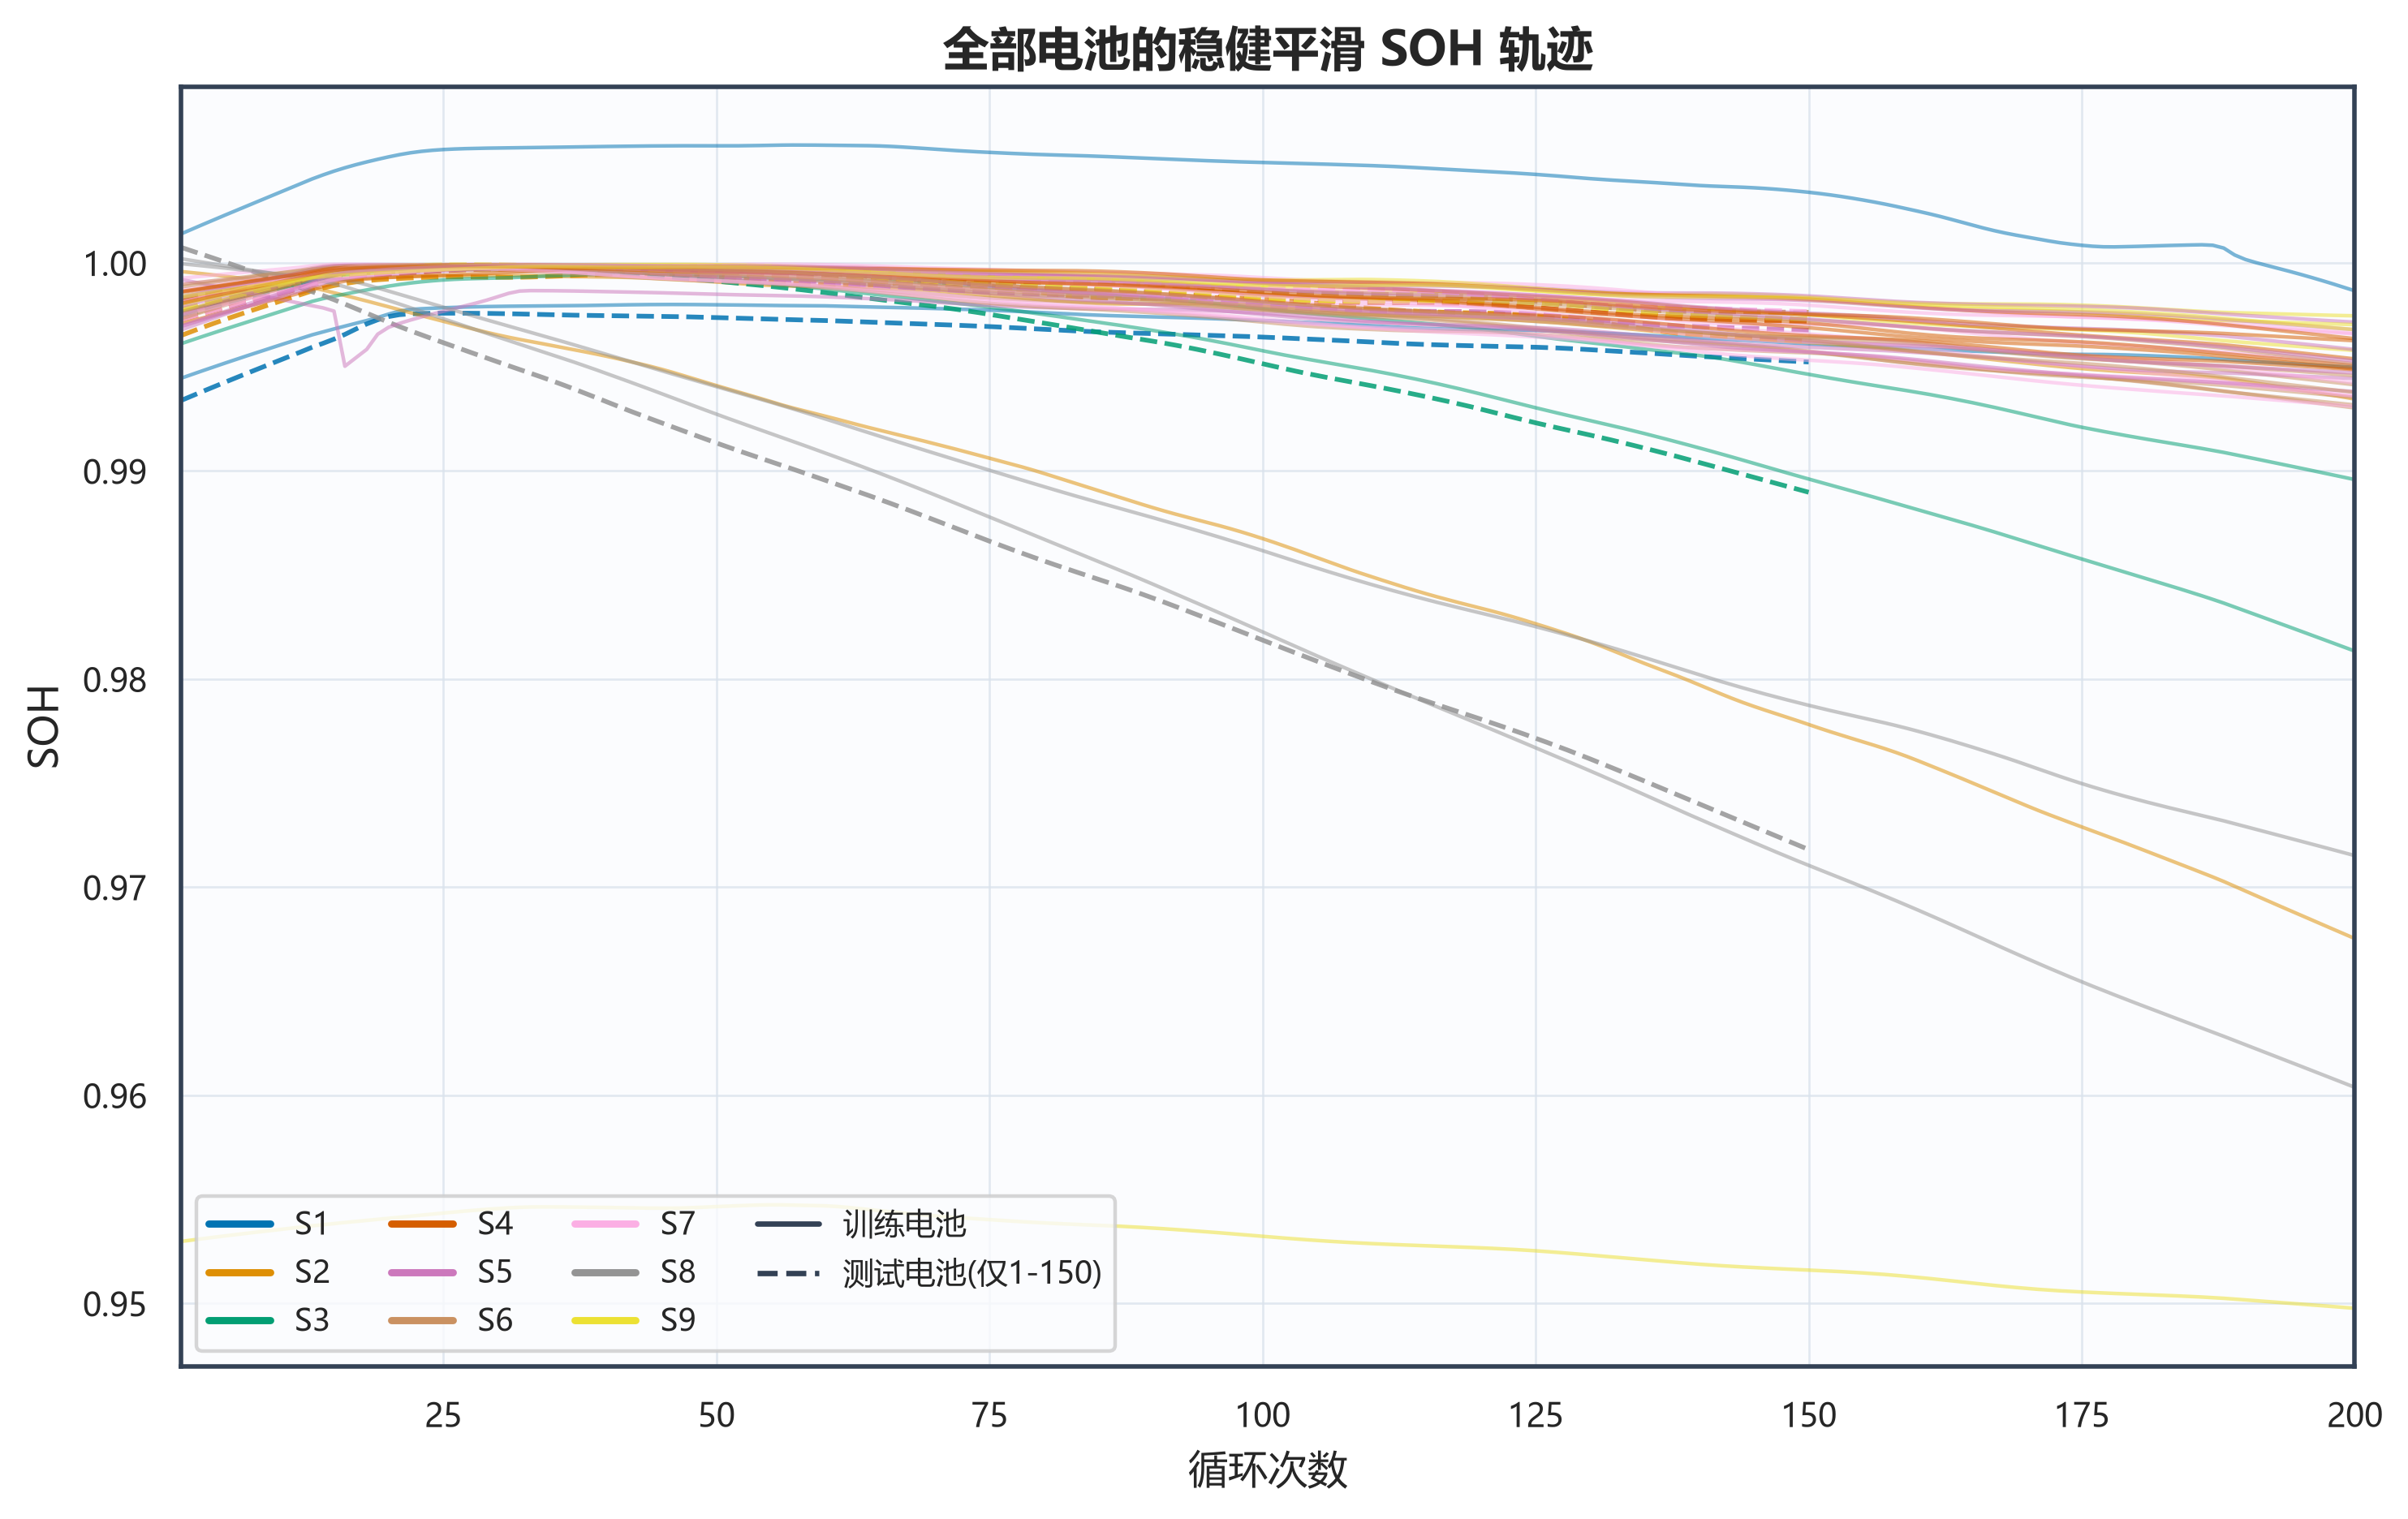
\includegraphics[width=0.96\textwidth]{q1_01_all_battery_soh_curves.png}
\caption{全部电池 SOH 曲线及充电策略分组}
\label{fig:q1all}
\end{figure}

\section{问题一：SOH 退化模型与循环寿命估计}\label{sec:q1}

\subsection{候选模型与物理约束}

令 $z=t/100$，比较下列低参数模型：
\begin{align}
  \text{Linear: }&f(z)=a-dz,\quad d\ge0,\\
  \text{Quadratic: }&f(z)=a-d_1z-d_2z^2,\quad d_1,d_2\ge0,\\
  \text{Power: }&f(z)=a-dz^r,\quad d\ge0,r>0,\\
  \text{Exponential: }&f(z)=a-d\{\exp(rz)-1\},\quad d,r\ge0.
\end{align}
参数使用 soft-$L_1$ 损失估计，以降低残余局部波动的影响。所有候选均约束长期总体单调不增，避免高阶多项式反弹。寿命定义为
\[
  \widehat L_i=\min\{t\ge1:f_i(t/100)\le0.8\},
\]
搜索上限为 5000 次；无法稳定过阈值时不强制报告确定值。

\subsection{时间截断验证与模型选择}

对每块训练电池分别用 1--100 次预测 101--200 次、用 1--150 次预测 151--200 次。验证指标为 MAE、RMSE、最大绝对误差、未来趋势方向和 100/150/200 次拟合所得 EOL 的稳定性。该设计直接模拟可用早期数据预测未来，而不是随机拆分循环行。

\begin{table}[H]
\centering
\caption{最终受约束二次模型的截断验证结果}
\begin{tabular}{ccccc}
\toprule
截断点 & 中位 MAE & 中位 RMSE & 中位 MaxAE & 趋势一致率 \\
\midrule
100 & 0.000786 & 0.000909 & 0.001997 & 97.5\% \\
150 & 0.000312 & 0.000366 & 0.000770 & 100.0\% \\
\bottomrule
\end{tabular}
\end{table}

综合误差、趋势、EOL 稳定性和可解释性，受约束二次模型的综合选择得分最低（1.37），故作为统一寿命口径。图\ref{fig:q1model}给出典型短、中、长寿命电池的拟合与外推；图\ref{fig:q1valid}表明选择依据是短期外推而非训练集 $R^2$。

\begin{figure}[H]
\centering
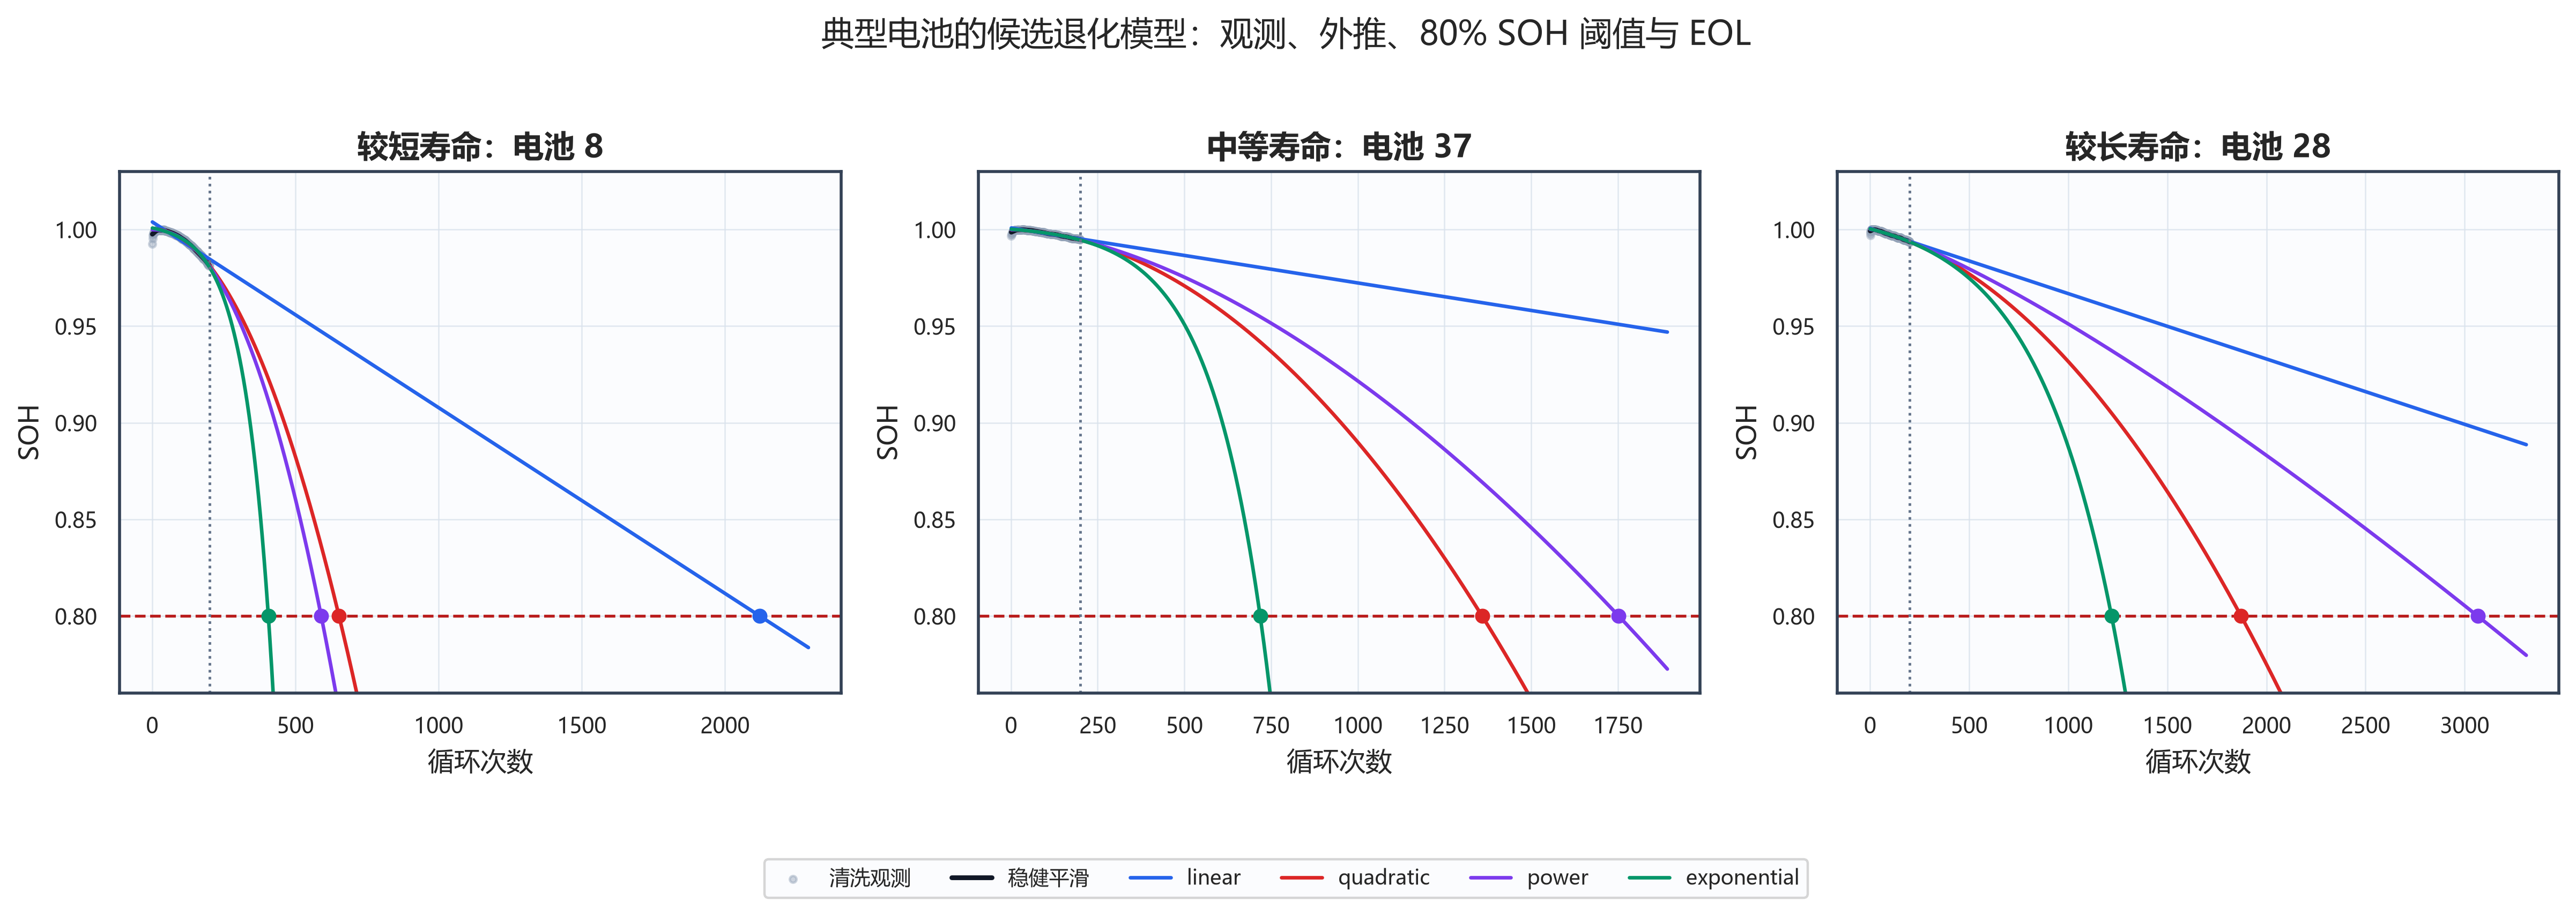
\includegraphics[width=0.95\textwidth]{q1_11_typical_model_extrapolations.png}
\caption{典型电池的候选模型拟合、外推与 80\% SOH 阈值}
\label{fig:q1model}
\end{figure}

\begin{figure}[H]
\centering
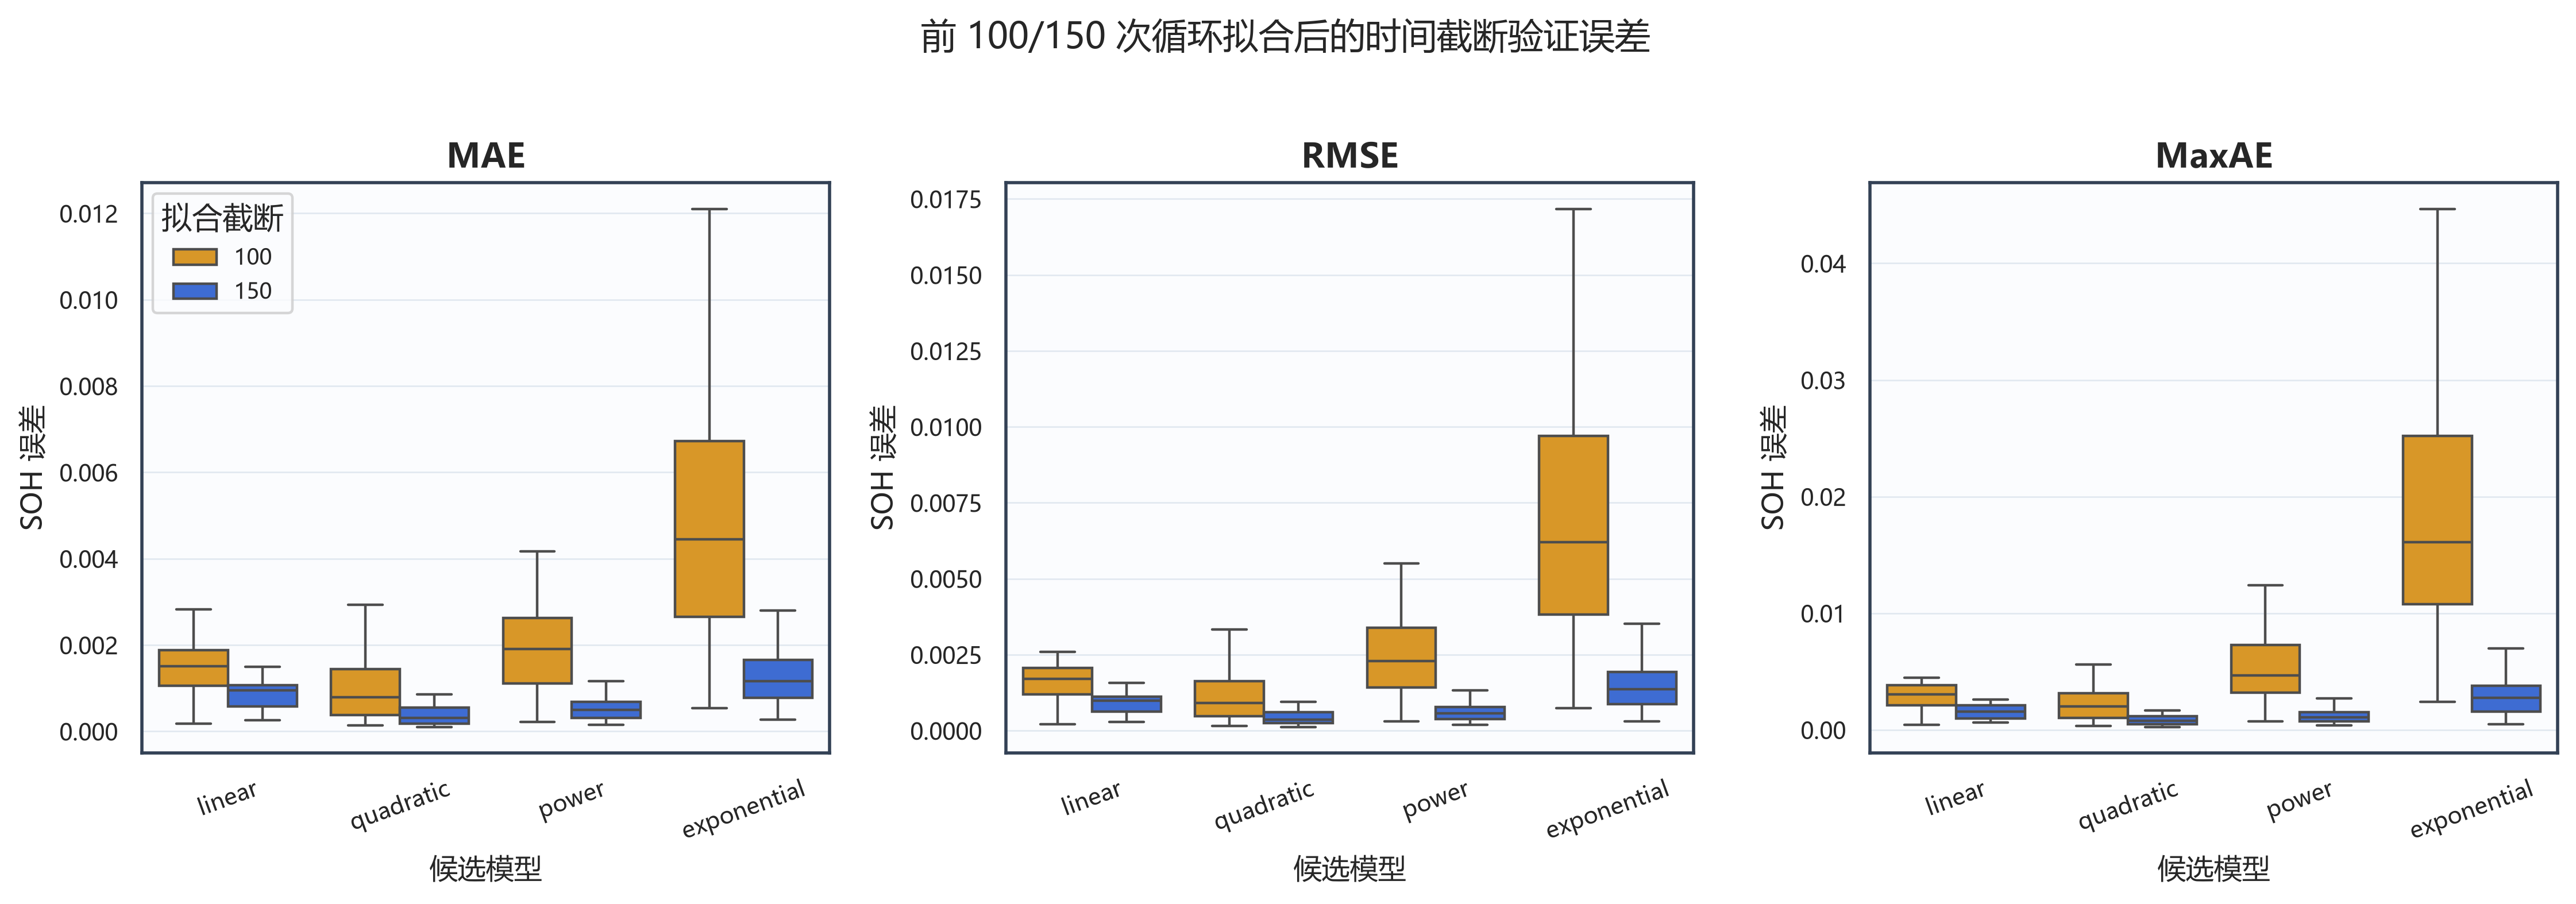
\includegraphics[width=0.88\textwidth]{q1_12_truncation_validation_errors.png}
\caption{候选模型的时间截断验证误差}
\label{fig:q1valid}
\end{figure}

\subsection{寿命估计及策略聚合}

40 块训练电池的二次模型 EOL 估计范围为 652.5--1872.2 次，中位数 1348.7 次。采用 300 次移动块残差 bootstrap\cite{efron1979} 传播参数与残差不确定性，99.7\% 以上的重采样可获得有限 EOL；区间宽度与点估计之比的中位数为 19.4\%。由 150 次扩展到 200 次后，EOL 相对变化的中位数为 5.11\%，说明排序具有一定稳定性，但绝对寿命仍受模型结构影响：40 块电池中仅 1 块达到条件稳定等级，其余 39 块为中高结构敏感。

\begin{table}[H]
\centering
\caption{各策略早期退化与条件性 EOL 汇总（中位数）}
\resizebox{\textwidth}{!}{
\begin{tabular}{ccccccc}
\toprule
策略 & 训练电池数 & SOH$_{150}$ & SOH$_{200}$ & 50--200 斜率/100次 & EOL/次 & 观察性特征 \\
\midrule
S1 & 2 & 0.999745 & 0.996815 & $-0.002785$ & 1407.8 & 下降较慢 \\
S2 & 2 & 0.986989 & 0.980490 & $-0.010561$ & 930.7 & 下降较快 \\
S3 & 2 & 0.992125 & 0.985461 & $-0.009321$ & 776.1 & EOL点估计较低 \\
S4 & 6 & 0.997309 & 0.995217 & $-0.003033$ & 1362.4 & 组内较稳定 \\
S5 & 7 & 0.997295 & 0.995289 & $-0.002874$ & 1426.1 & 组内较稳定 \\
S6 & 7 & 0.996287 & 0.993772 & $-0.003583$ & 1333.2 & 中等 \\
S7 & 7 & 0.996580 & 0.994226 & $-0.003551$ & 1473.7 & 中等偏好 \\
S8 & 2 & 0.974889 & 0.965946 & $-0.018560$ & 1017.3 & 早期退化最明显 \\
S9 & 5 & 0.998221 & 0.996789 & $-0.002000$ & 1649.2 & 点估计较高 \\
\bottomrule
\end{tabular}}
\end{table}

早期斜率与 EOL 的 Spearman 相关为 0.77，SOH$_{200}$ 与 EOL 的相关为 0.66；由于两者来自同一 SOH 曲线，这些相关只说明指标一致性，不能作为独立验证。策略寿命分布见图\ref{fig:q1life}。

\begin{figure}[H]
\centering
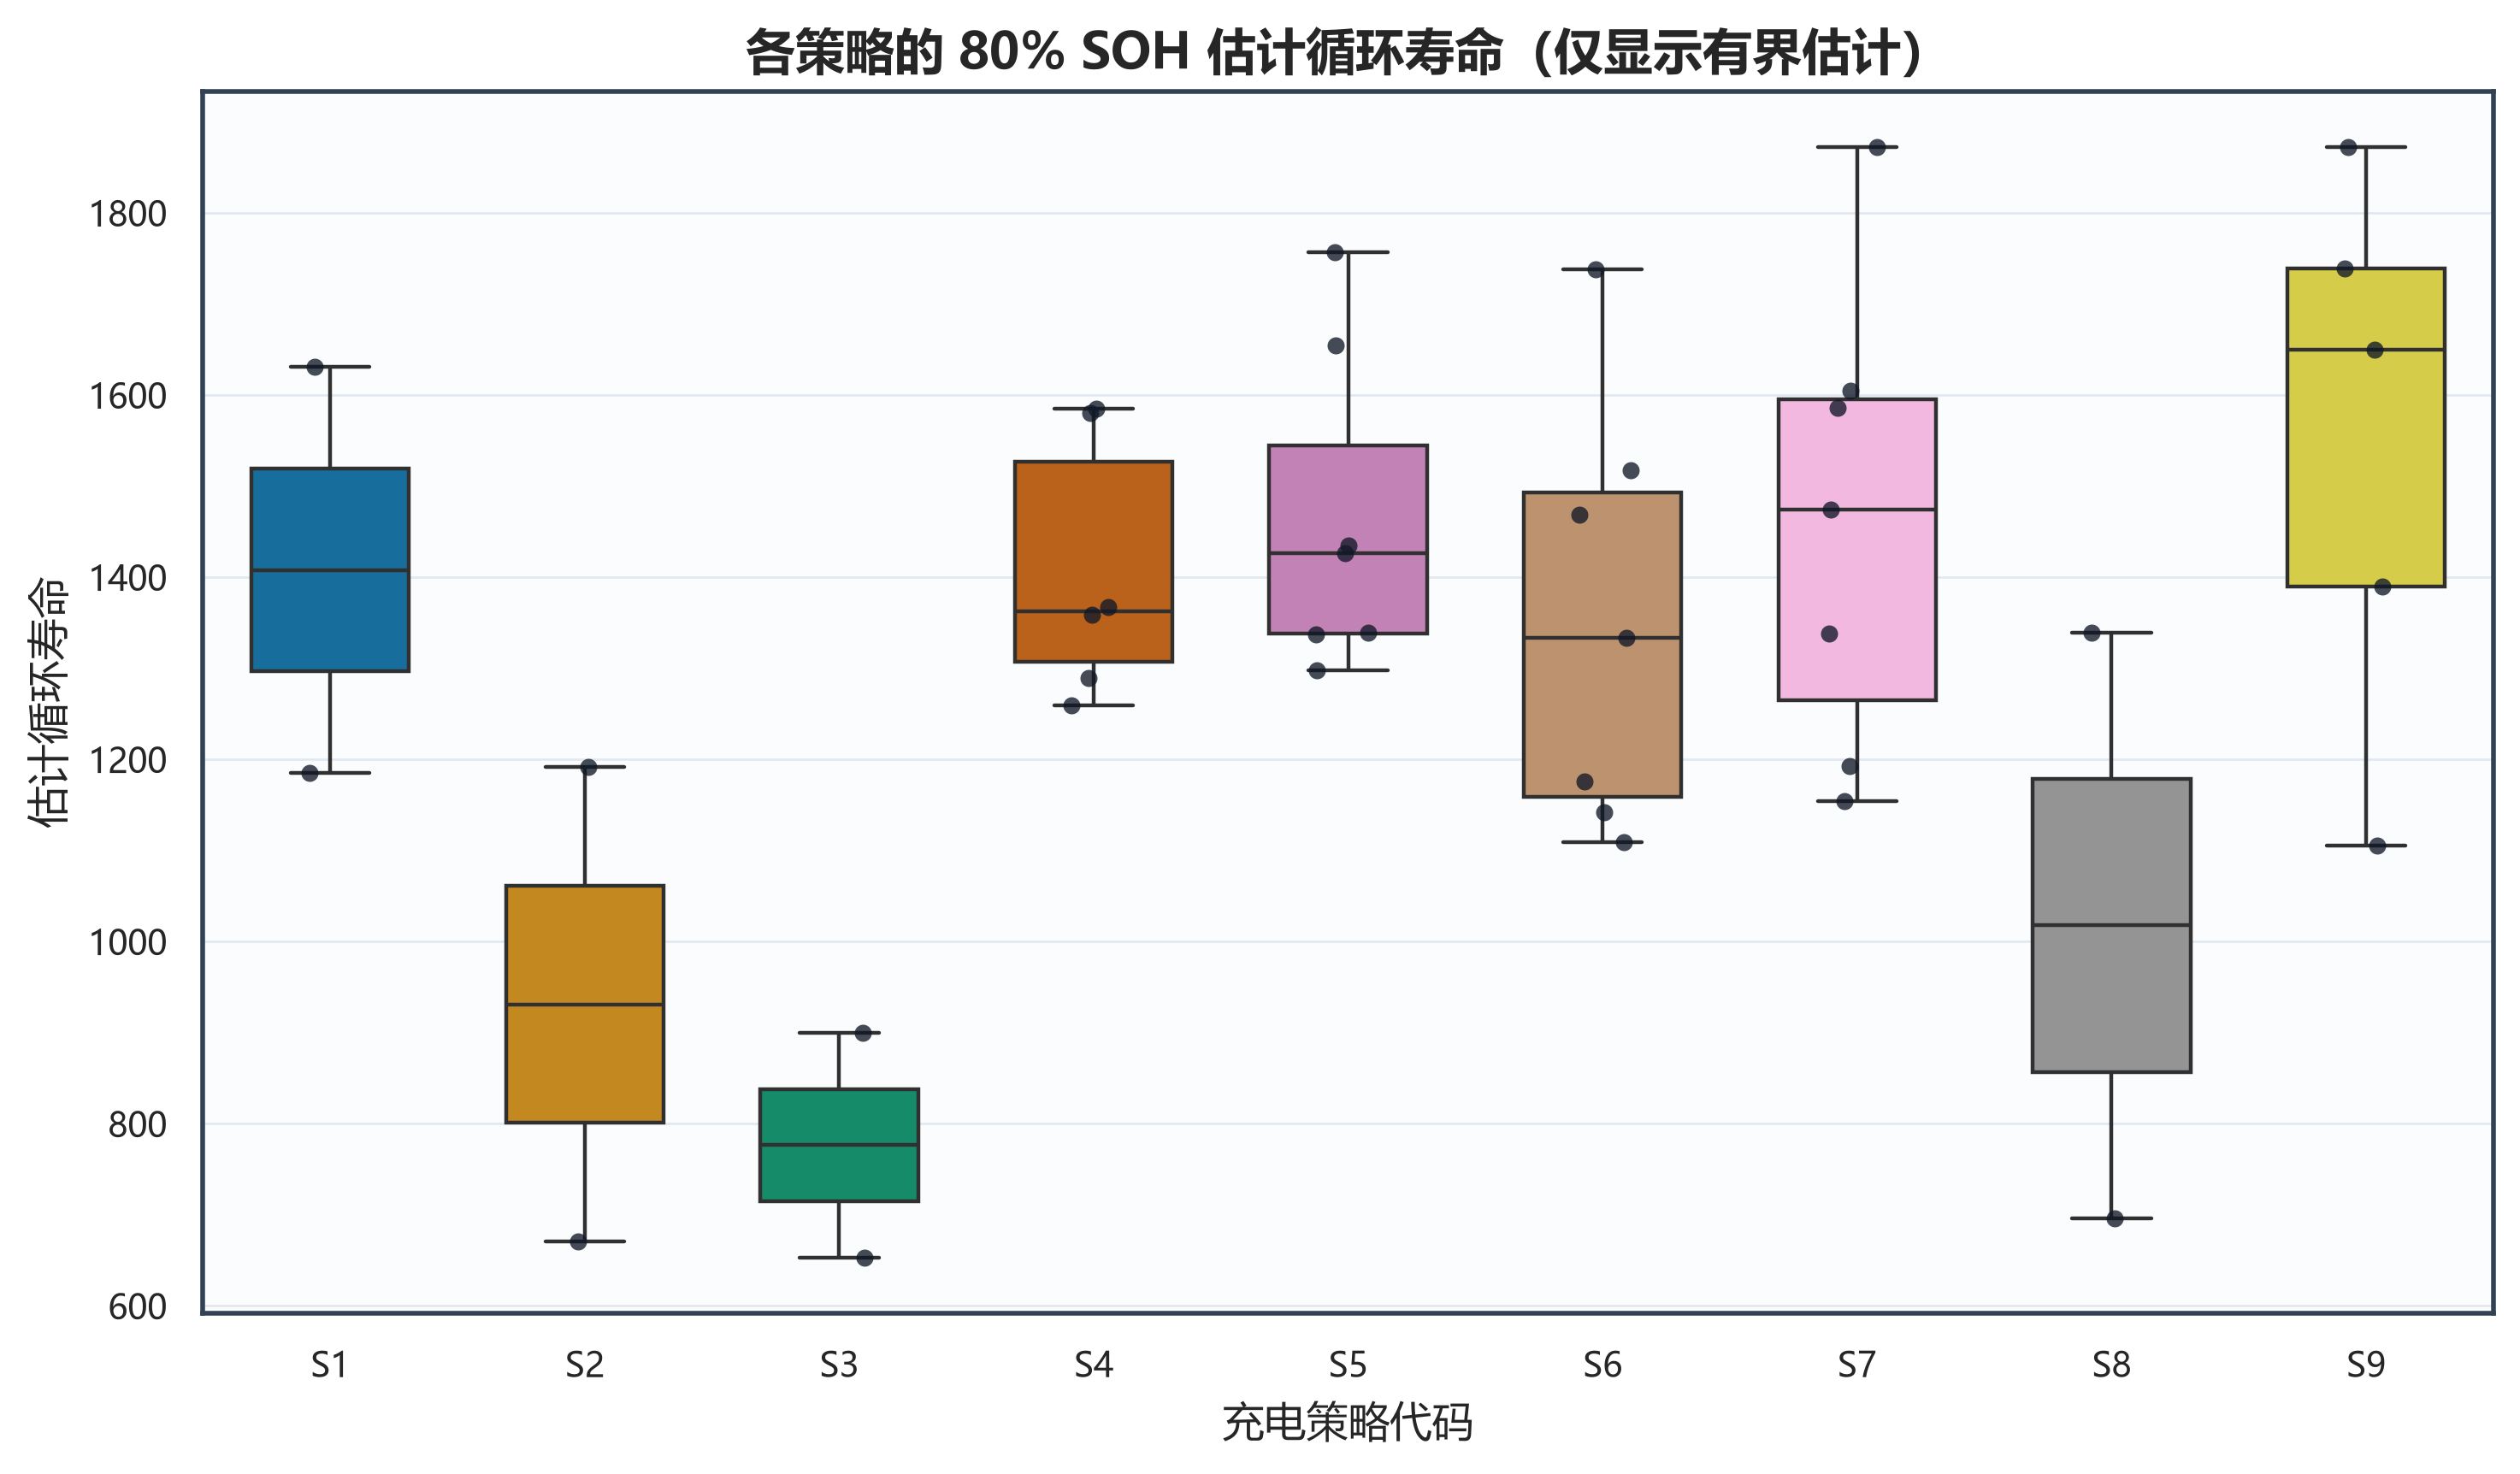
\includegraphics[width=0.82\textwidth]{q1_08_estimated_life_by_strategy.png}
\caption{各策略条件性 EOL 分布与单电池散点}
\label{fig:q1life}
\end{figure}

\section{问题二：充电策略参数与退化的统计关系}\label{sec:q2}

\subsection{策略整体差异的稳健检验}

以电池为基本单位，对 SOH$_{150}$、SOH$_{200}$、$D$、曲率及 EOL 同时实施 Welch 检验\cite{welch1951}、Kruskal--Wallis 检验\cite{kruskal1952}和 19999 次策略标签置换。效应量报告 $\eta^2$ 及 Cliff's delta\cite{cliff1993}；若总体检验显著，再作成对置换并以 Holm 法\cite{holm1979}校正。bootstrap 按策略整组重采样，避免把同一策略内的循环记录当成独立样本。

\begin{table}[H]
\centering
\caption{策略整体差异的主要置换检验结果}
\begin{tabular}{lccc}
\toprule
响应 & 置换 $p$ 值 & $\eta^2$ & 解释 \\
\midrule
SOH$_{150}$ & 0.04780 & 0.3869 & 总体差异边界显著 \\
SOH$_{200}$ & 0.01955 & 0.4817 & 总体差异显著 \\
50--200 退化率 & 0.00015 & 0.7944 & 差异强且方向清晰 \\
退化曲率 & 0.00020 & 0.7476 & 差异强 \\
条件性 EOL & 0.00815 & 0.4697 & 总体差异显著但受外推影响 \\
\bottomrule
\end{tabular}
\end{table}

总体差异显著不等于任意两策略都可区分；受每组仅 2--7 块电池限制，Holm 校正后的成对比较均未达到 0.05。图\ref{fig:q2dist}显示 S8 在 SOH$_{200}$ 与退化率上与其他策略方向一致地较差，是可靠的描述性发现；各精确策略排名仍受组内离散度限制。

\begin{figure}[H]
\centering
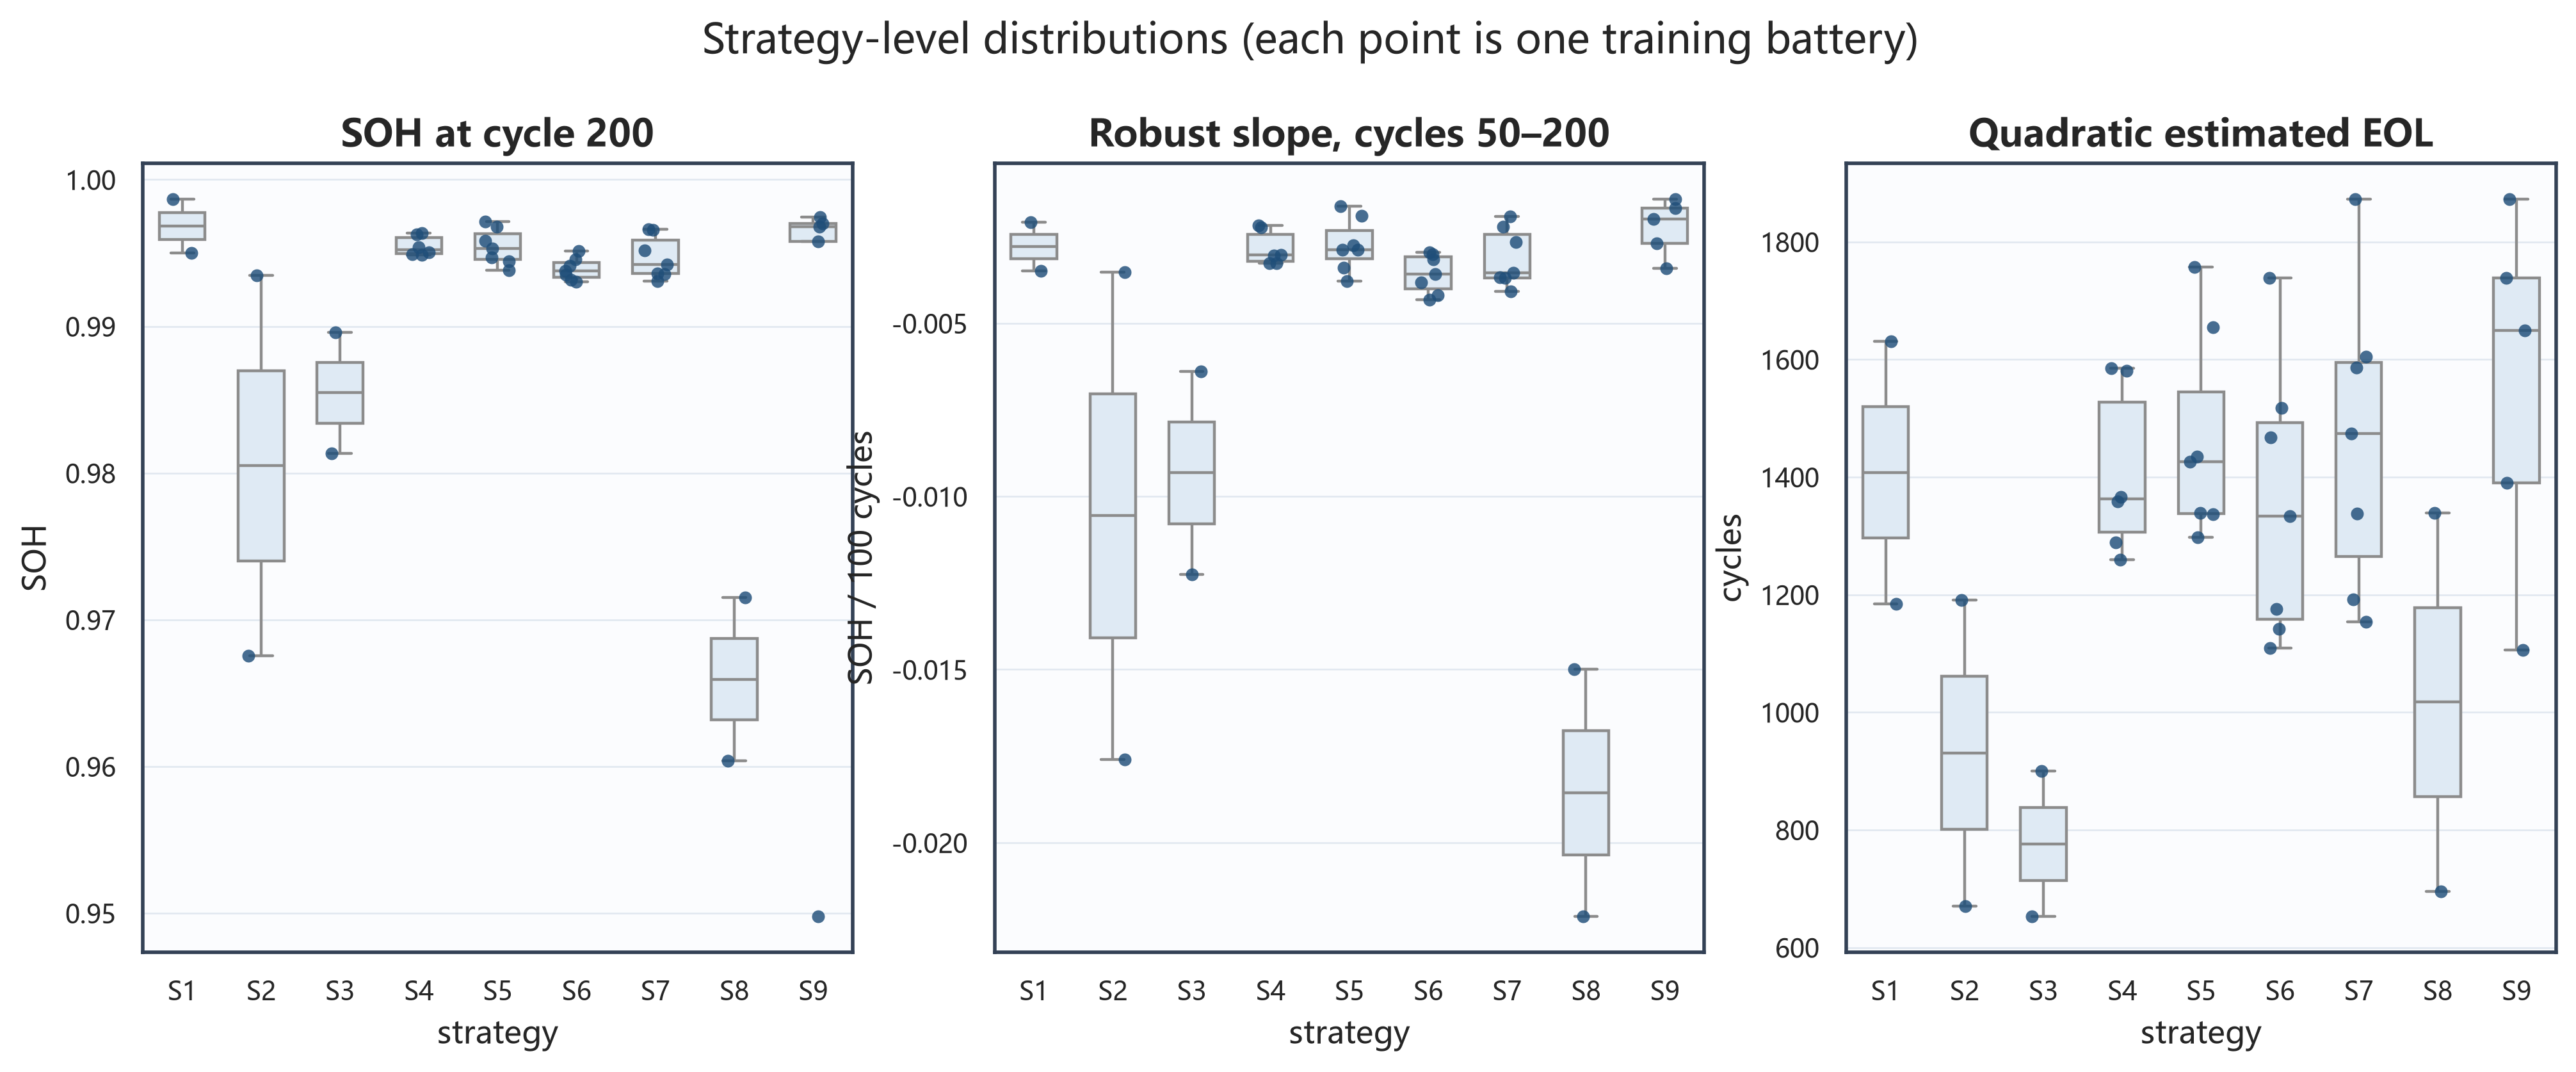
\includegraphics[width=0.95\textwidth]{q2_01_strategy_primary_distributions.png}
\caption{各策略 SOH$_{200}$、早期退化率与 EOL 的分布}
\label{fig:q2dist}
\end{figure}

\subsection{参数回归、共线性与批次敏感性}

策略 \texttt{80PER\_3\_6C} 的 $C_1$ 缺失，参数回归中排除、分类比较中保留。对其余 8 个策略先拟合
\[
  Y=\beta_0+\beta_1C_1+\beta_2Q_1+\beta_3C_2+\varepsilon,
\]
并用标准化岭回归\cite{hoerl1970}作稳定性对照。全数据 VIF 为 1.37--1.51，但 dataset 3 内 $C_1,C_2$ 的 VIF 增至 5.51、6.13，最大相关系数为 0.823。因 NEWSTRUCTURE 与 dataset 3 完全重合，strategy 与 batch 不能完全分离。

全样本 OLS 中 $C_2$ 对 SOH$_{200}$ 和斜率的标准化系数约为 $-0.669$、$-0.665$，但加入批次变量或仅保留 dataset 3 后系数可显著缩小甚至变号，所有分组 bootstrap 区间均跨 0。单变量层面，$C_2$ 与 SOH$_{200}$ 的 Spearman $\rho=-0.699$、$p=0.0623$，与斜率的 $\rho=-0.566$、$p=0.150$；$C_1$ 未显示“越高必然退化越快”的单调证据。故较高 $C_2$ 只可表述为不利趋势，不能解释成独立因果效应。

\subsection{SOC 加权应力}

构造
\[
  S_p=\frac{Q_1}{80}C_1^p+\frac{80-Q_1}{80}C_2^p,\qquad 1\le p\le3.
\]
该指标把倍率大小与持续 SOC 区间合并，且参数数目受控。交叉验证在预设范围边界选择 $p=3$，但 $p=2\sim3$ 性能接近，不能把 3 视作确定物理指数。dataset 3 内应力模型对观察性退化指标的拟合方向一致，S8 的应力最高且退化最严重；然而应力与二次 EOL 的 Spearman $\rho=-0.060$、$p=0.899$，说明长期寿命关系对外推结构敏感。

\begin{figure}[H]
\centering
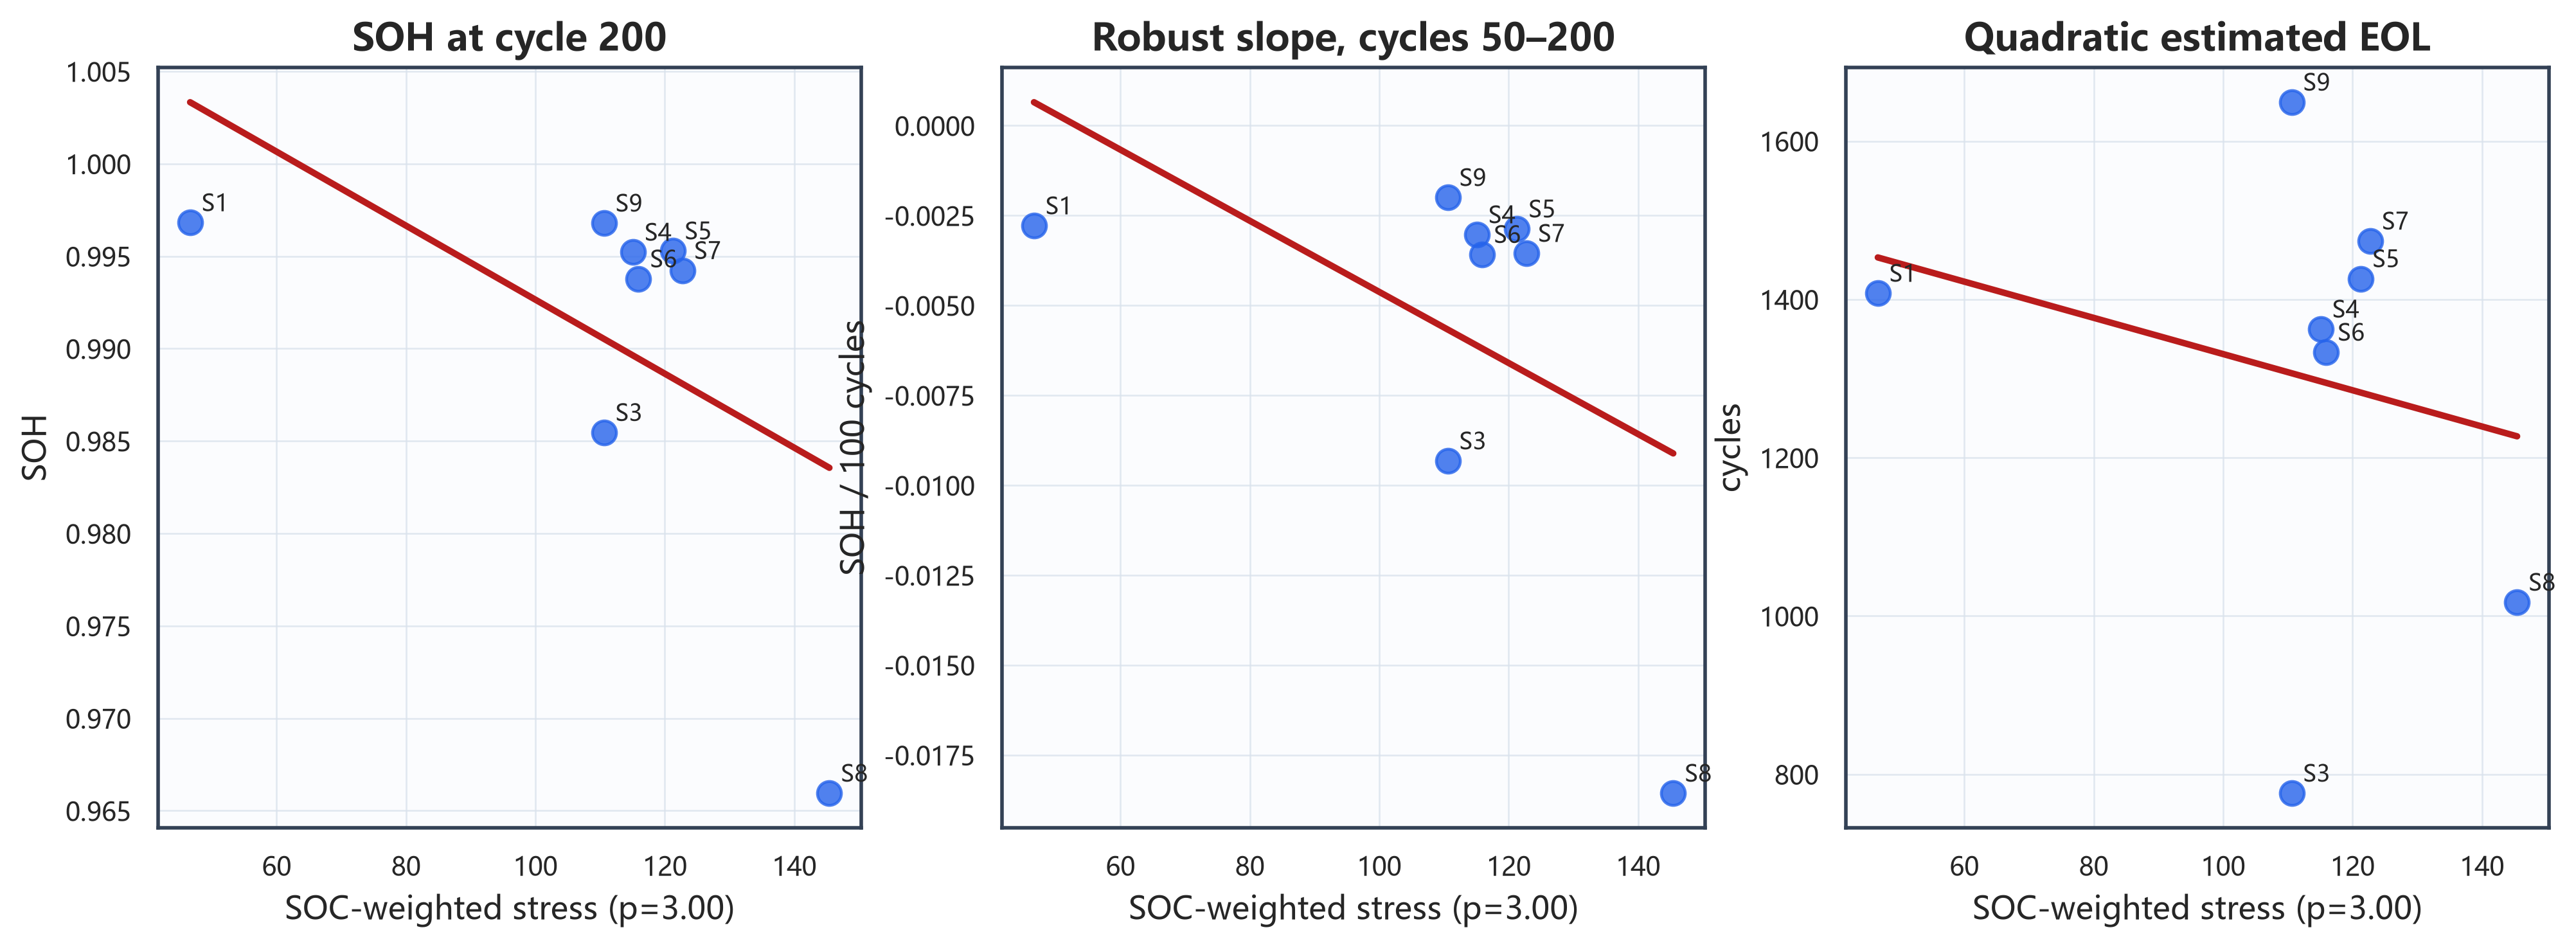
\includegraphics[width=0.92\textwidth]{q2_05_stress_primary_relations.png}
\caption{SOC 加权应力与多类退化响应的关系}
\label{fig:q2stress}
\end{figure}

综上，稳定结论是策略整体早期退化存在差异且 S8 较差；趋势性结论是中高 SOC 阶段维持高倍率可能更不利；受限结论是 $C_1,Q_1,C_2$ 的独立效应及应力--EOL 关系，二者均受策略点少、共线性、批次和寿命模型结构约束。

\section{问题三：测试电池第 151--200 次 SOH 与 EOL 预测}\label{sec:q3}

\subsection{严格伪测试设计}

按最新赛题补充，40 块非测试电池截至第 200 次的全部已提供观测均可用于问题三的训练、参数拟合和验证。本文对每块训练电池轮流设为伪测试对象：在第 $i$ 个外层折中，仅向模型暴露目标电池 $i$ 的 1--150 次，并将其真实 151--200 次保留为验证标签；其余 39 块训练电池可使用 1--200 次，分别构造策略群体模板、拟合监督模型和选择参数。目标电池的未来段同时从策略模板、监督模型、标准化器、岭参数选择、集成权重及区间校准中排除。完成伪测试和模型选择后，再使用全部 40 块非测试电池的 1--200 次重新拟合群体模板与监督模型，并应用于 9 块测试电池。测试电池在任何阶段都不使用 150 次以后的信息，也不利用 global ID 查询外部寿命。这里的“全部已提供观测”不等于真实完整生命周期，第 200 次以后的 EOL 仍需外推。

候选模型包括：单电池受约束二次外推；100--150 次局部 Theil--Sen 趋势；同策略留一平均模板；群体模板加个体残差修正；以前 150 次特征预测未来形状系数的岭回归。对目标电池 $i$，个体修正写为
\[
  \widehat y_i(t)=\mu_{p,-i}(t)+\hat\alpha_i+hat\gamma_i(t-150)+\hat\kappa_i(t-150)^2,
\]
其中曲率施加轻度正则。再按训练电池交叉验证误差形成自适应集成：
\[
  \widehat y_i^{\rm ens}(t)=\sum_m w_{im}\widehat y_{im}(t),\qquad
  w_{im}\propto\{e_m^2(1+\lambda z_i)\}^{-1}.
\]
$z_i$ 综合 SOH$_{150}$、100--150 次斜率、内阻趋势和模板残差。偏离同策略群体越大，模板权重越低、个体模型权重越高。

\subsection{伪测试性能与模型选择}

\begin{table}[H]
\centering
\caption{最终自适应集成的严格伪测试性能}
\begin{tabular}{lc}
\toprule
指标 & 数值 \\
\midrule
电池级平均 MAE & 0.000277 \\
电池级平均 RMSE & 0.000361 \\
电池级中位 MAE & 0.000196 \\
电池级 MAE 的 90\% 分位数 & 0.000901 \\
最差电池 MAE & 0.002912 \\
cycle 200 平均绝对误差 & 0.000522 \\
未来趋势方向一致率 & 100\% \\
策略级 MAE 标准差 & 0.000516 \\
\bottomrule
\end{tabular}
\end{table}

局部线性模型的平均 RMSE 为 0.000393、cycle 200 MAE 为 0.000604；集成分别降低 8.2\% 和 13.6\%。它没有依赖单一复杂黑箱，而是通过群体形状减少单电池外推方差，再由个体残差和偏离度校正模板偏差。总体真实--预测轨迹见图\ref{fig:q3overall}，模型误差分布见图\ref{fig:q3errors}。

\begin{figure}[H]
\centering
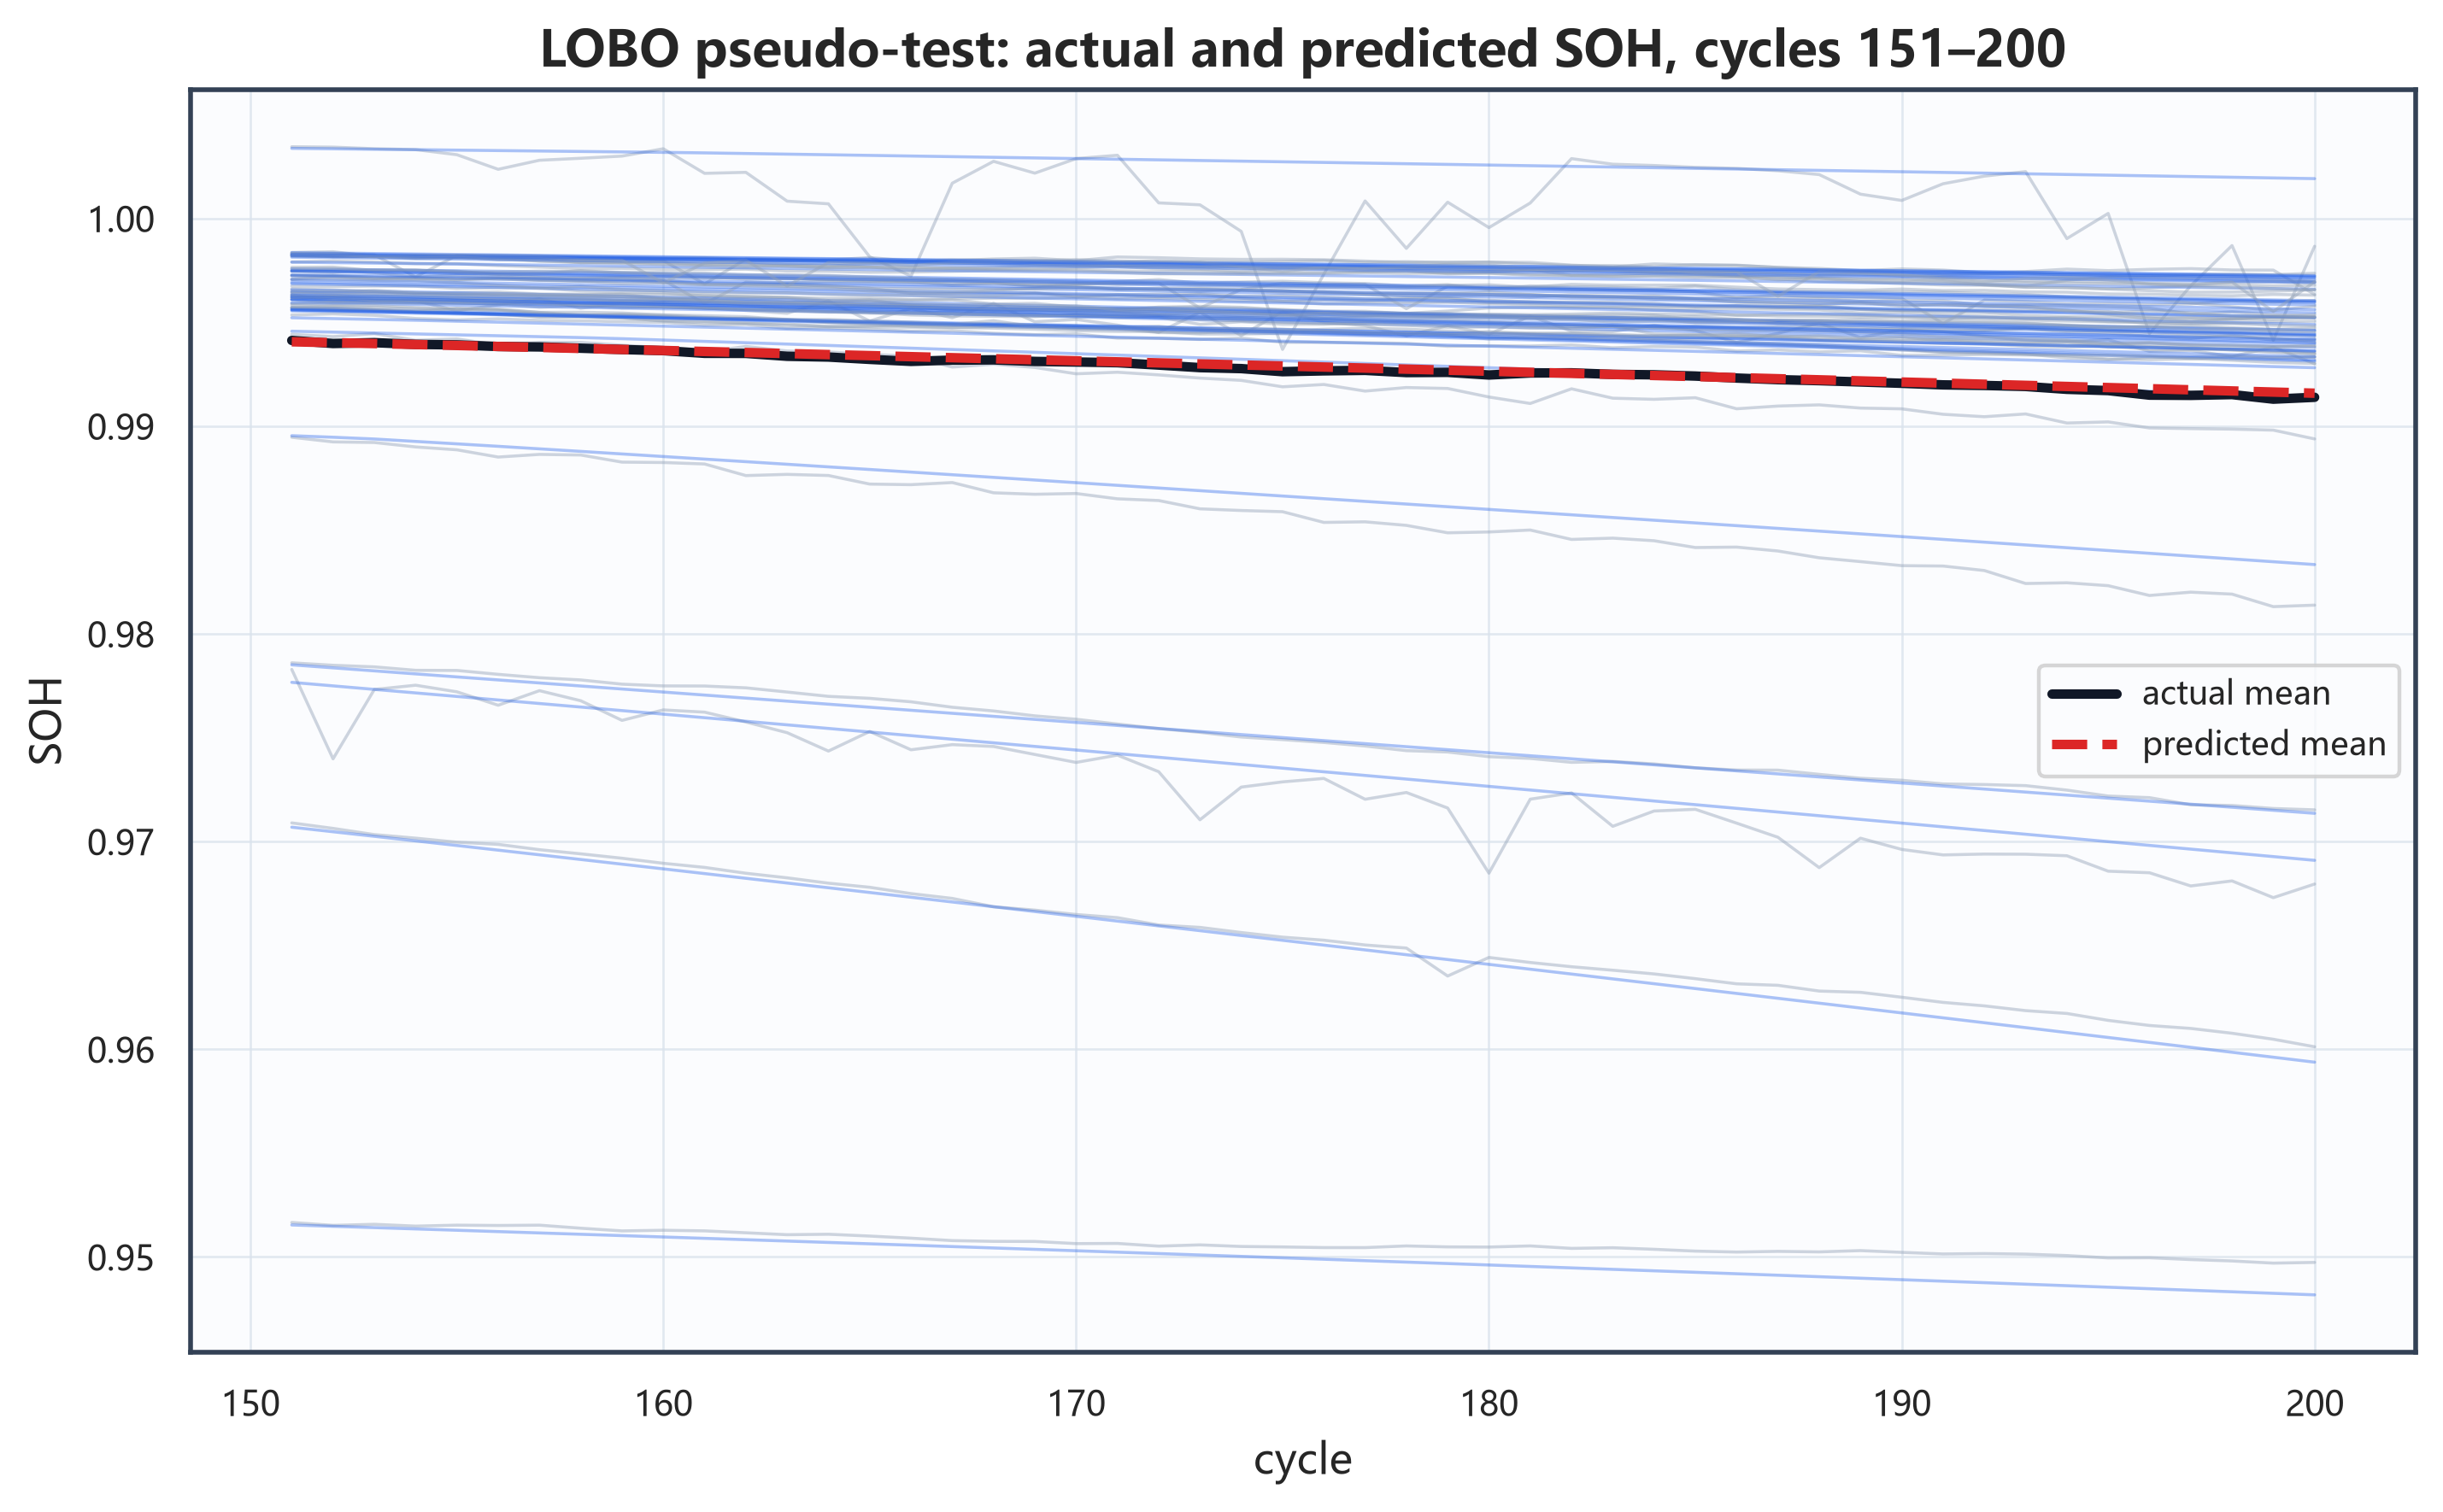
\includegraphics[width=0.94\textwidth]{q3_01_pseudotest_all_actual_vs_predicted.png}
\caption{40 块训练电池严格伪测试的真实与预测轨迹}
\label{fig:q3overall}
\end{figure}

\begin{figure}[H]
\centering
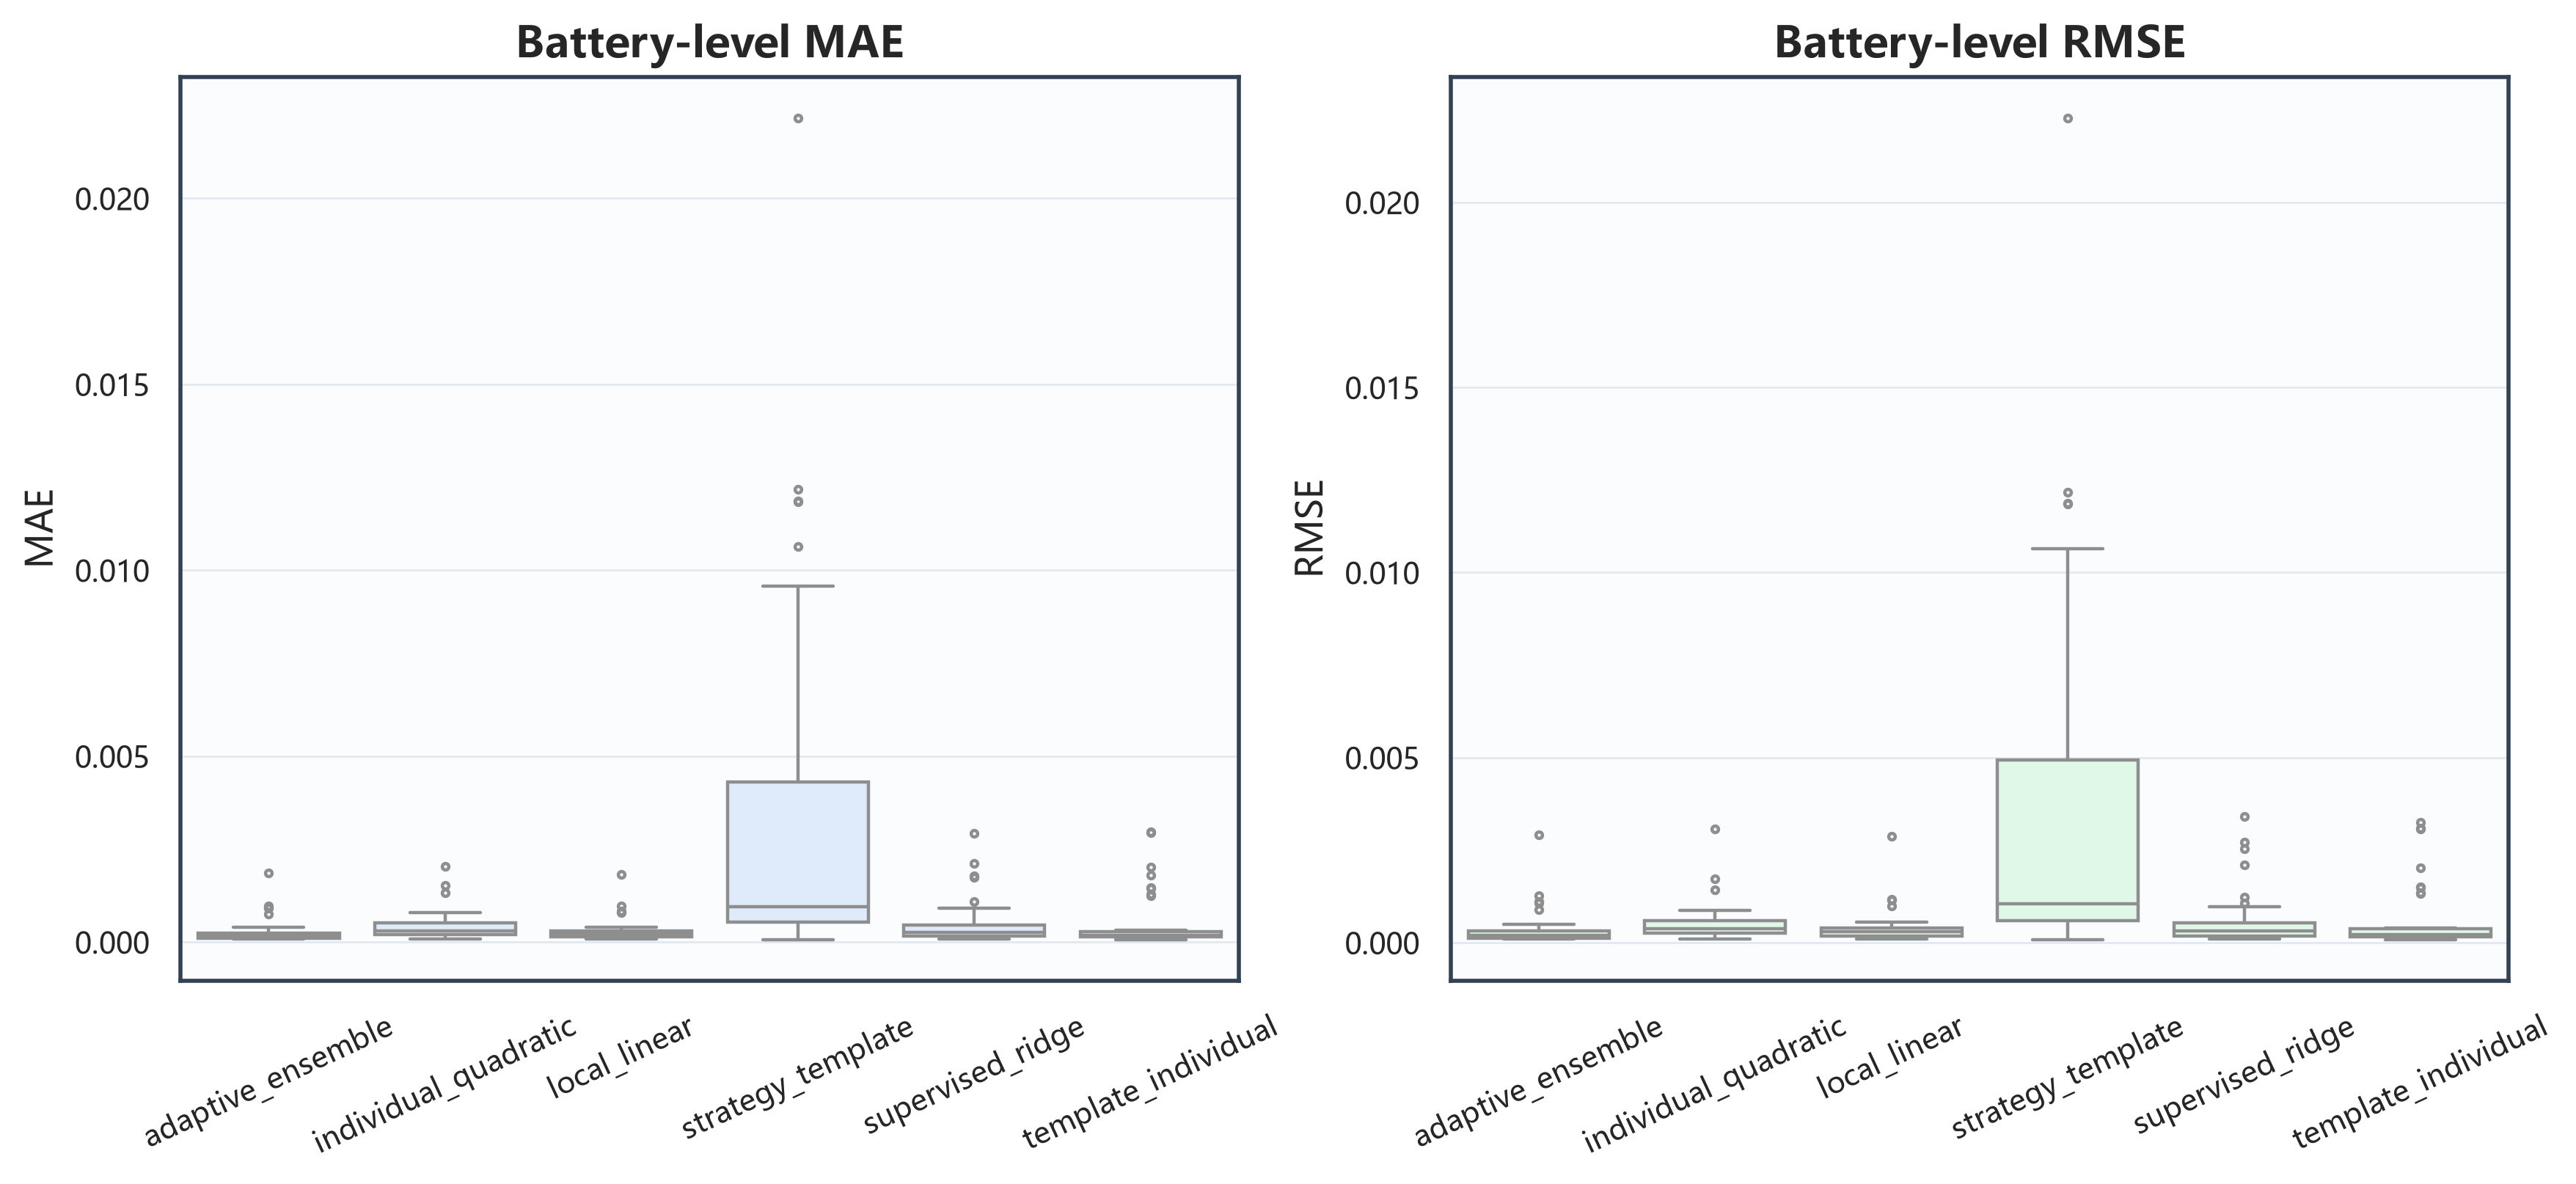
\includegraphics[width=0.88\textwidth]{q3_03_model_error_distributions.png}
\caption{候选模型 MAE 与 RMSE 分布}
\label{fig:q3errors}
\end{figure}

预测区间由逐预测步长的留一绝对残差 95\% 分位数、模型分歧和个体偏离度共同形成。训练电池区间的平均覆盖率为 95.9\%，中位数为 100\%，但最差电池仅 48\%，因此区间是经验校准而非严格概率保证。

\subsection{9 块测试电池预测结果}

\begin{table}[H]
\centering
\caption{测试电池 cycle 200 与条件性 EOL 预测}
\resizebox{\textwidth}{!}{
\begin{tabular}{ccccccc}
\toprule
电池 & 策略 & $\widehat{\SOH}_{200}$ & 95\%经验区间 & EOL点估计/次 & EOL区间/次 & 可靠性 \\
\midrule
B2  & S1 & 0.993555 & [0.990378,0.996732] & 1412.8 & [928.6,1479.9] & 中低 \\
B5  & S2 & 0.993762 & [0.989958,0.997566] & 1169.8 & [902.3,1291.3] & 中低 \\
B9  & S3 & 0.982127 & [0.978541,0.985713] & 657.1 & [589.6,671.6] & 中低 \\
B10 & S4 & 0.995481 & [0.993060,0.997902] & 1388.8 & [975.8,1473.8] & 中低 \\
B11 & S5 & 0.994963 & [0.992448,0.997479] & 1532.4 & [1035.3,2684.9] & 低 \\
B14 & S6 & 0.995942 & [0.993555,0.998329] & 1436.1 & [993.7,1883.0] & 低 \\
B16 & S8 & 0.962507 & [0.959468,0.965545] & 1003.2 & [628.5,1051.7] & 相对高$^*$ \\
B24 & S7 & 0.995993 & [0.993673,0.998314] & 1433.5 & [894.0,1565.5] & 中低 \\
B25 & S9 & 0.995706 & [0.992244,0.999168] & 1467.6 & [976.6,1704.8] & 低 \\
\bottomrule
\multicolumn{7}{l}{\footnotesize $^*$仅表示在当前模型与策略模板条件下相对较稳定，不表示 EOL 已被真实验证。}
\end{tabular}}
\end{table}

B2、B5、B25 的群体偏离分数分别为 2.295、2.688、4.380，已自动降低模板权重；B25 的寿命不确定性尤其受个体偏离和 S9 批次残差影响。B16 的短期下降最明显，但同策略形状较一致，因而其短期预测相对可靠。9 块电池的 151--200 次逐循环点预测和区间见图\ref{fig:q3test}。

\begin{figure}[H]
\centering
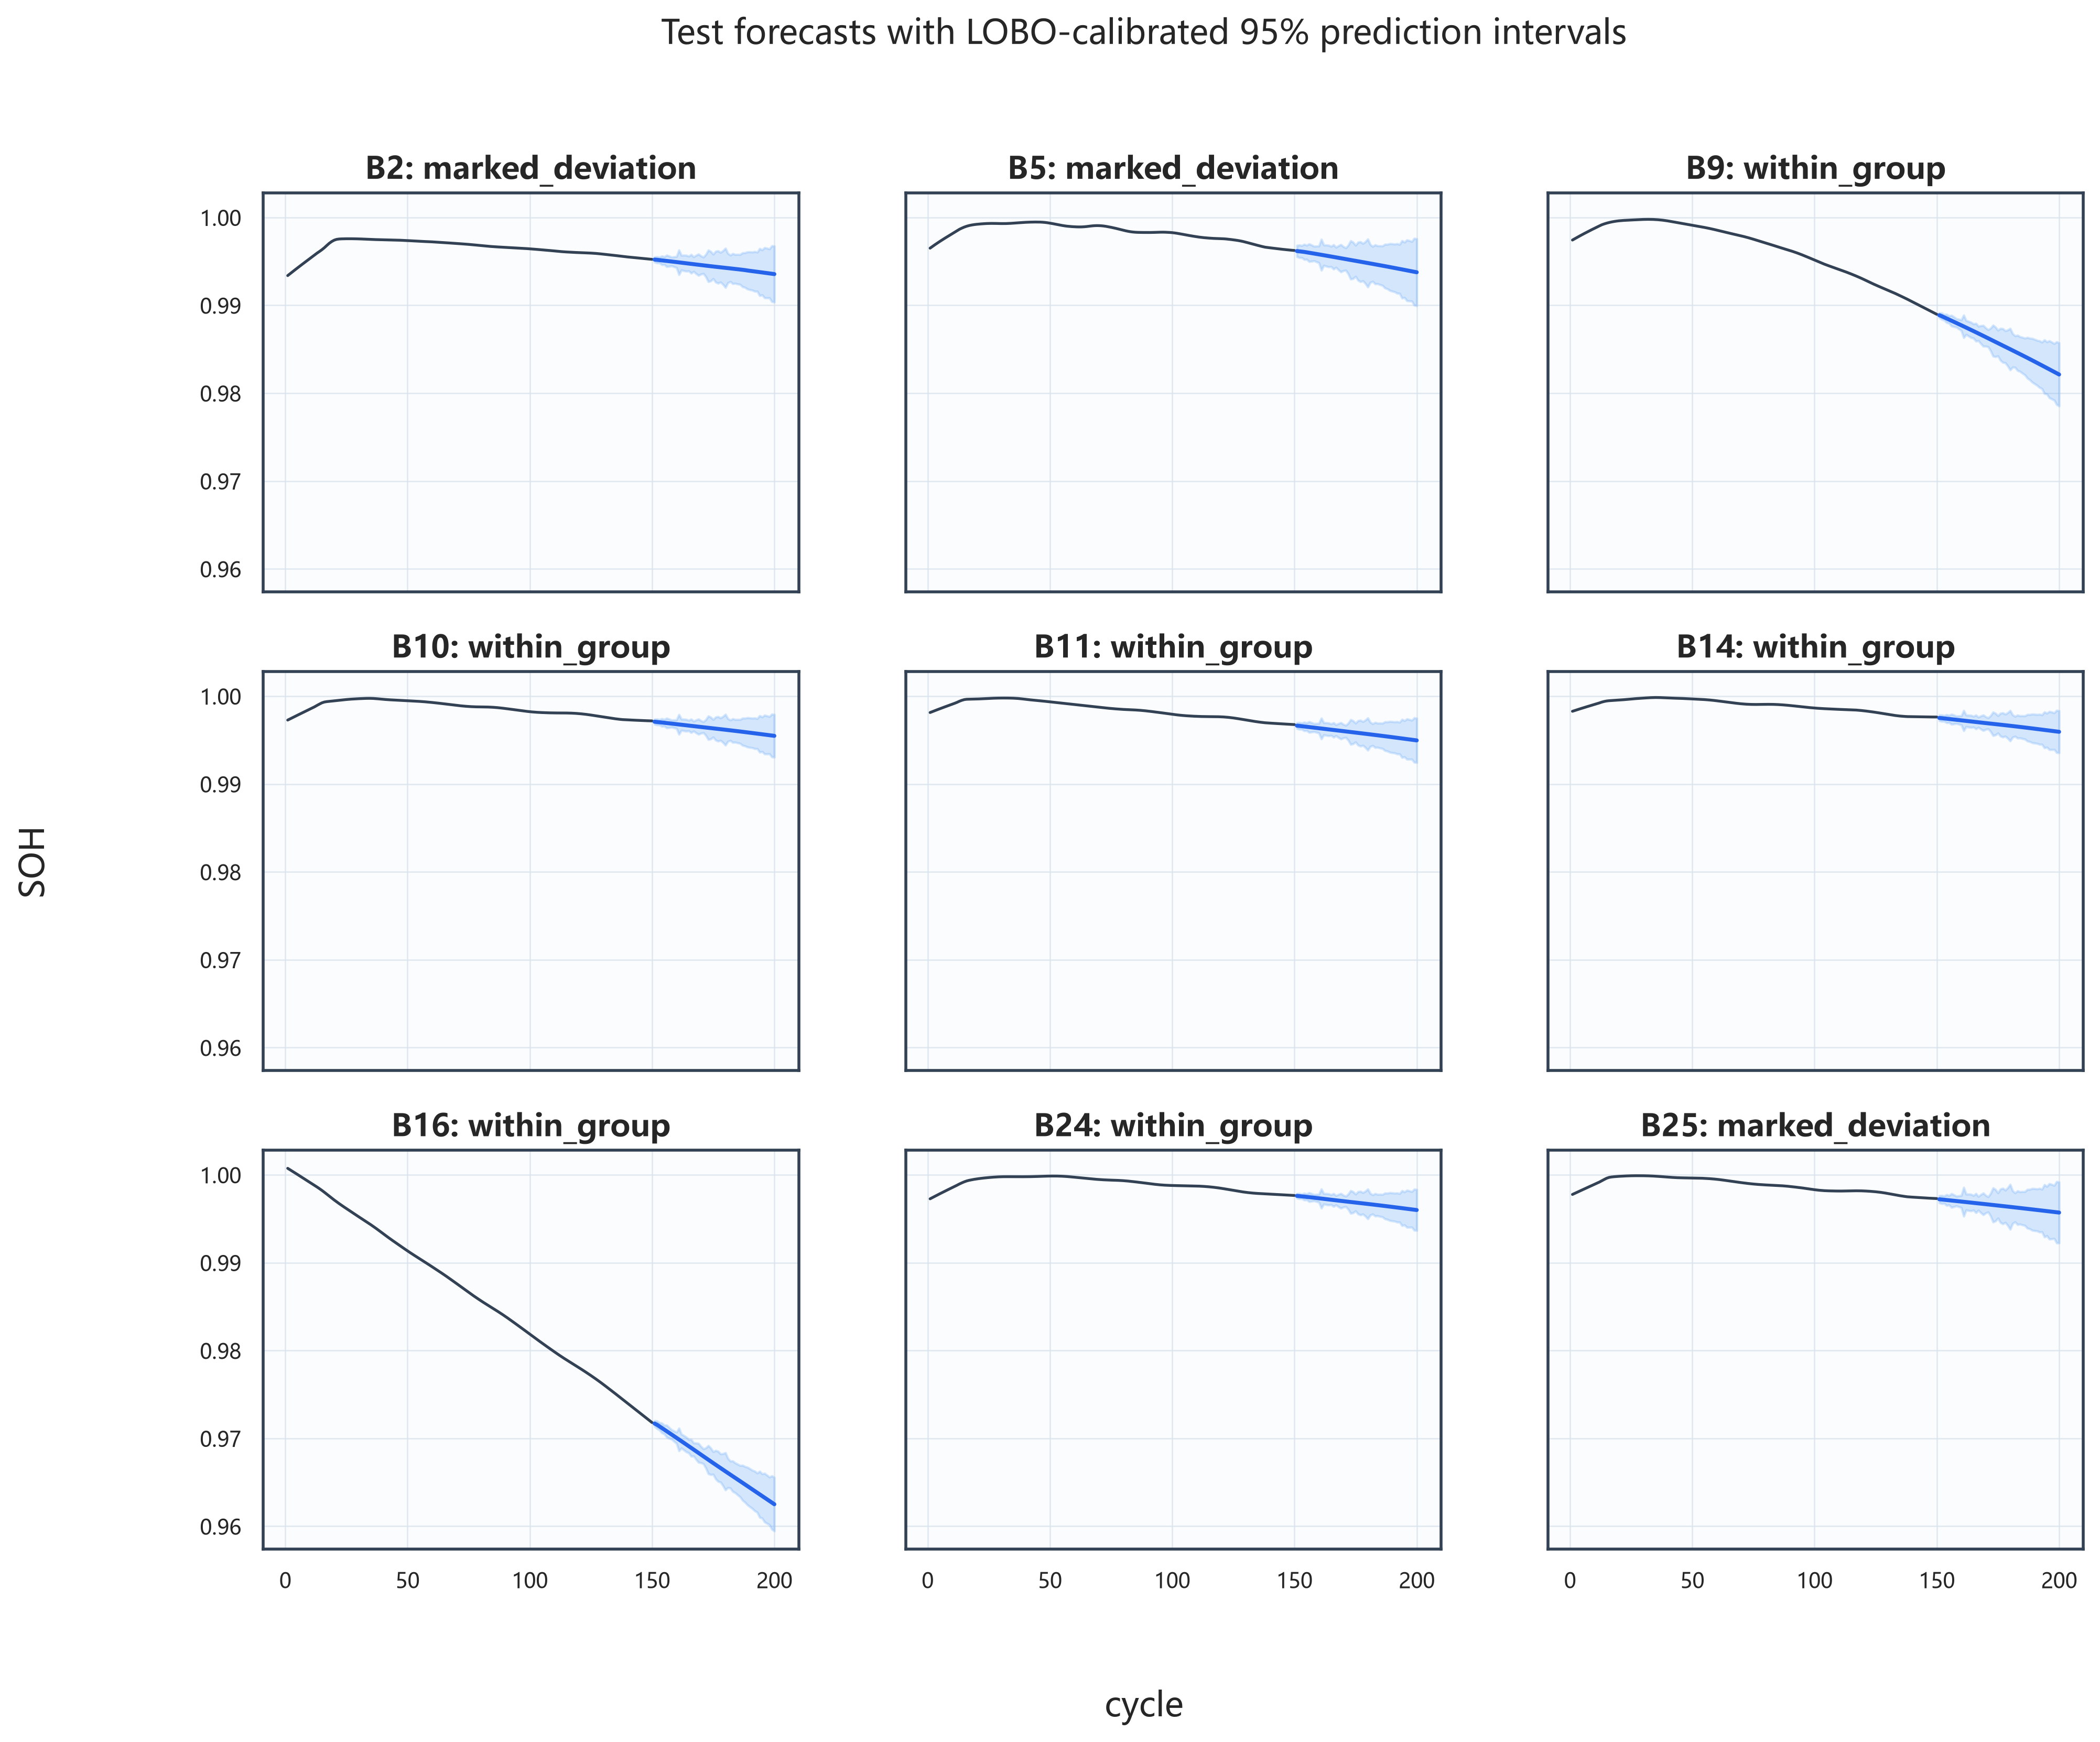
\includegraphics[width=0.96\textwidth]{q3_09_test_prediction_intervals.png}
\caption{9 块测试电池的观测段、预测段及经验区间}
\label{fig:q3test}
\end{figure}

EOL 采用“前 150 次实测 + 151--200 次预测 + 同策略群体轻度约束”后二次重拟合。在训练电池伪测试中，该方案相对完整 200 次二次模型的 EOL 差异中位数为 2.82\%，优于只用前 150 次的 5.07\%。不过完整 200 次模型本身也不是真实 EOL 标签，故这一结果只支持截断稳定性，不代表绝对寿命准确率。

\section{问题四：充电时间--退化多目标优化}\label{sec:q4}

\subsection{充电时间与退化代理}

两阶段恒流从 0\% 充至 80\% SOC 的理想时间由两段耗时相加：
\[
  T_{\rm ideal}(x)=60\left[\frac{Q_1/100}{C_1}+\frac{(80-Q_1)/100}{C_2}\right].
\]
仅在 dataset 3 / NEWSTRUCTURE 的 6 个参数完整策略上做留一策略验证。纯物理公式的 MAE、RMSE、MaxAE 为 0.224、0.429、1.039 min；“物理 + 常数偏移”的对应值为 0.326、0.439、0.978 min。二者 RMSE 仅差 2.4\%，按预设简约规则选择
\[
  \widehat T(x)=T_{\rm ideal}(x)+0.223708.
\]
更复杂的 $Q_1$ 线性、二次修正及仿射校准均未降低留一 RMSE。S9 存在约 1 min 的未解释残差，使时间模型 95\% 区间约为点估计上下 0.85 min。

退化主代理选用对观察性指标更稳健的 $D$，EOL 仅作辅助标注。对 $p\in\{2,2.5,3\}$ 比较单调对数线性模型
\begin{align}
  1-\widehat{\SOH}_{200}(x)&=\exp(a_S+b_SS_p(x)),\quad b_S\ge0,\\
  \widehat D(x)&=\exp(a_D+b_DS_p(x)),\quad b_D\ge0,\\
  \widehat L(x)&=\exp(a_L+b_LS_p(x)),\quad b_L\le0.
\end{align}
$p=2$ 的三响应平均归一化留一 RMSE 为 0.26695，$p=2.5,3$ 分别为 0.26765、0.26774，差异很小，因此 $p=2$ 只作为主分析设定。其 SOH$_{200}$、$D$、EOL 的留一 RMSE 分别为 0.00894、0.00461、146.8 次。

\subsection{可信域、Pareto 前沿与 knee}

dataset 3 的观测范围为 $C_1\in[3.7,5.6]$、$Q_1\in[19,80]$、$C_2\in[4.0,5.9]$。在步长 $(0.05,1,0.05)$ 的 94302 个网格点中，先要求
\[
  x\in\Omega=\mathcal H\cap\mathcal N,
\]
其中 $\mathcal H$ 为 6 个参数点的三维凸包，$\mathcal N$ 为标准化最近邻距离不超过阈值的信任域。6340 点位于凸包，4413 点同时满足两类约束。对 $\min(\widehat T,\widehat D)$ 作非支配筛选，得到 413 个 Pareto 候选。矩形域结果会落入实验支撑薄弱的角落，故不作为主推荐。

将 Pareto 两目标归一化后，以连接端点的弦为基准，取垂距最大的候选作为 knee：
\[
  x_{\rm knee}=\arg\max_{x\in\mathcal P}d\bigl((\widetilde T,\widetilde D),\ell_{\rm endpoints}\bigr).
\]
现有策略、可信候选及前沿见图\ref{fig:q4pareto}，三类代表方案见图\ref{fig:q4recommend}。

\begin{figure}[H]
\centering
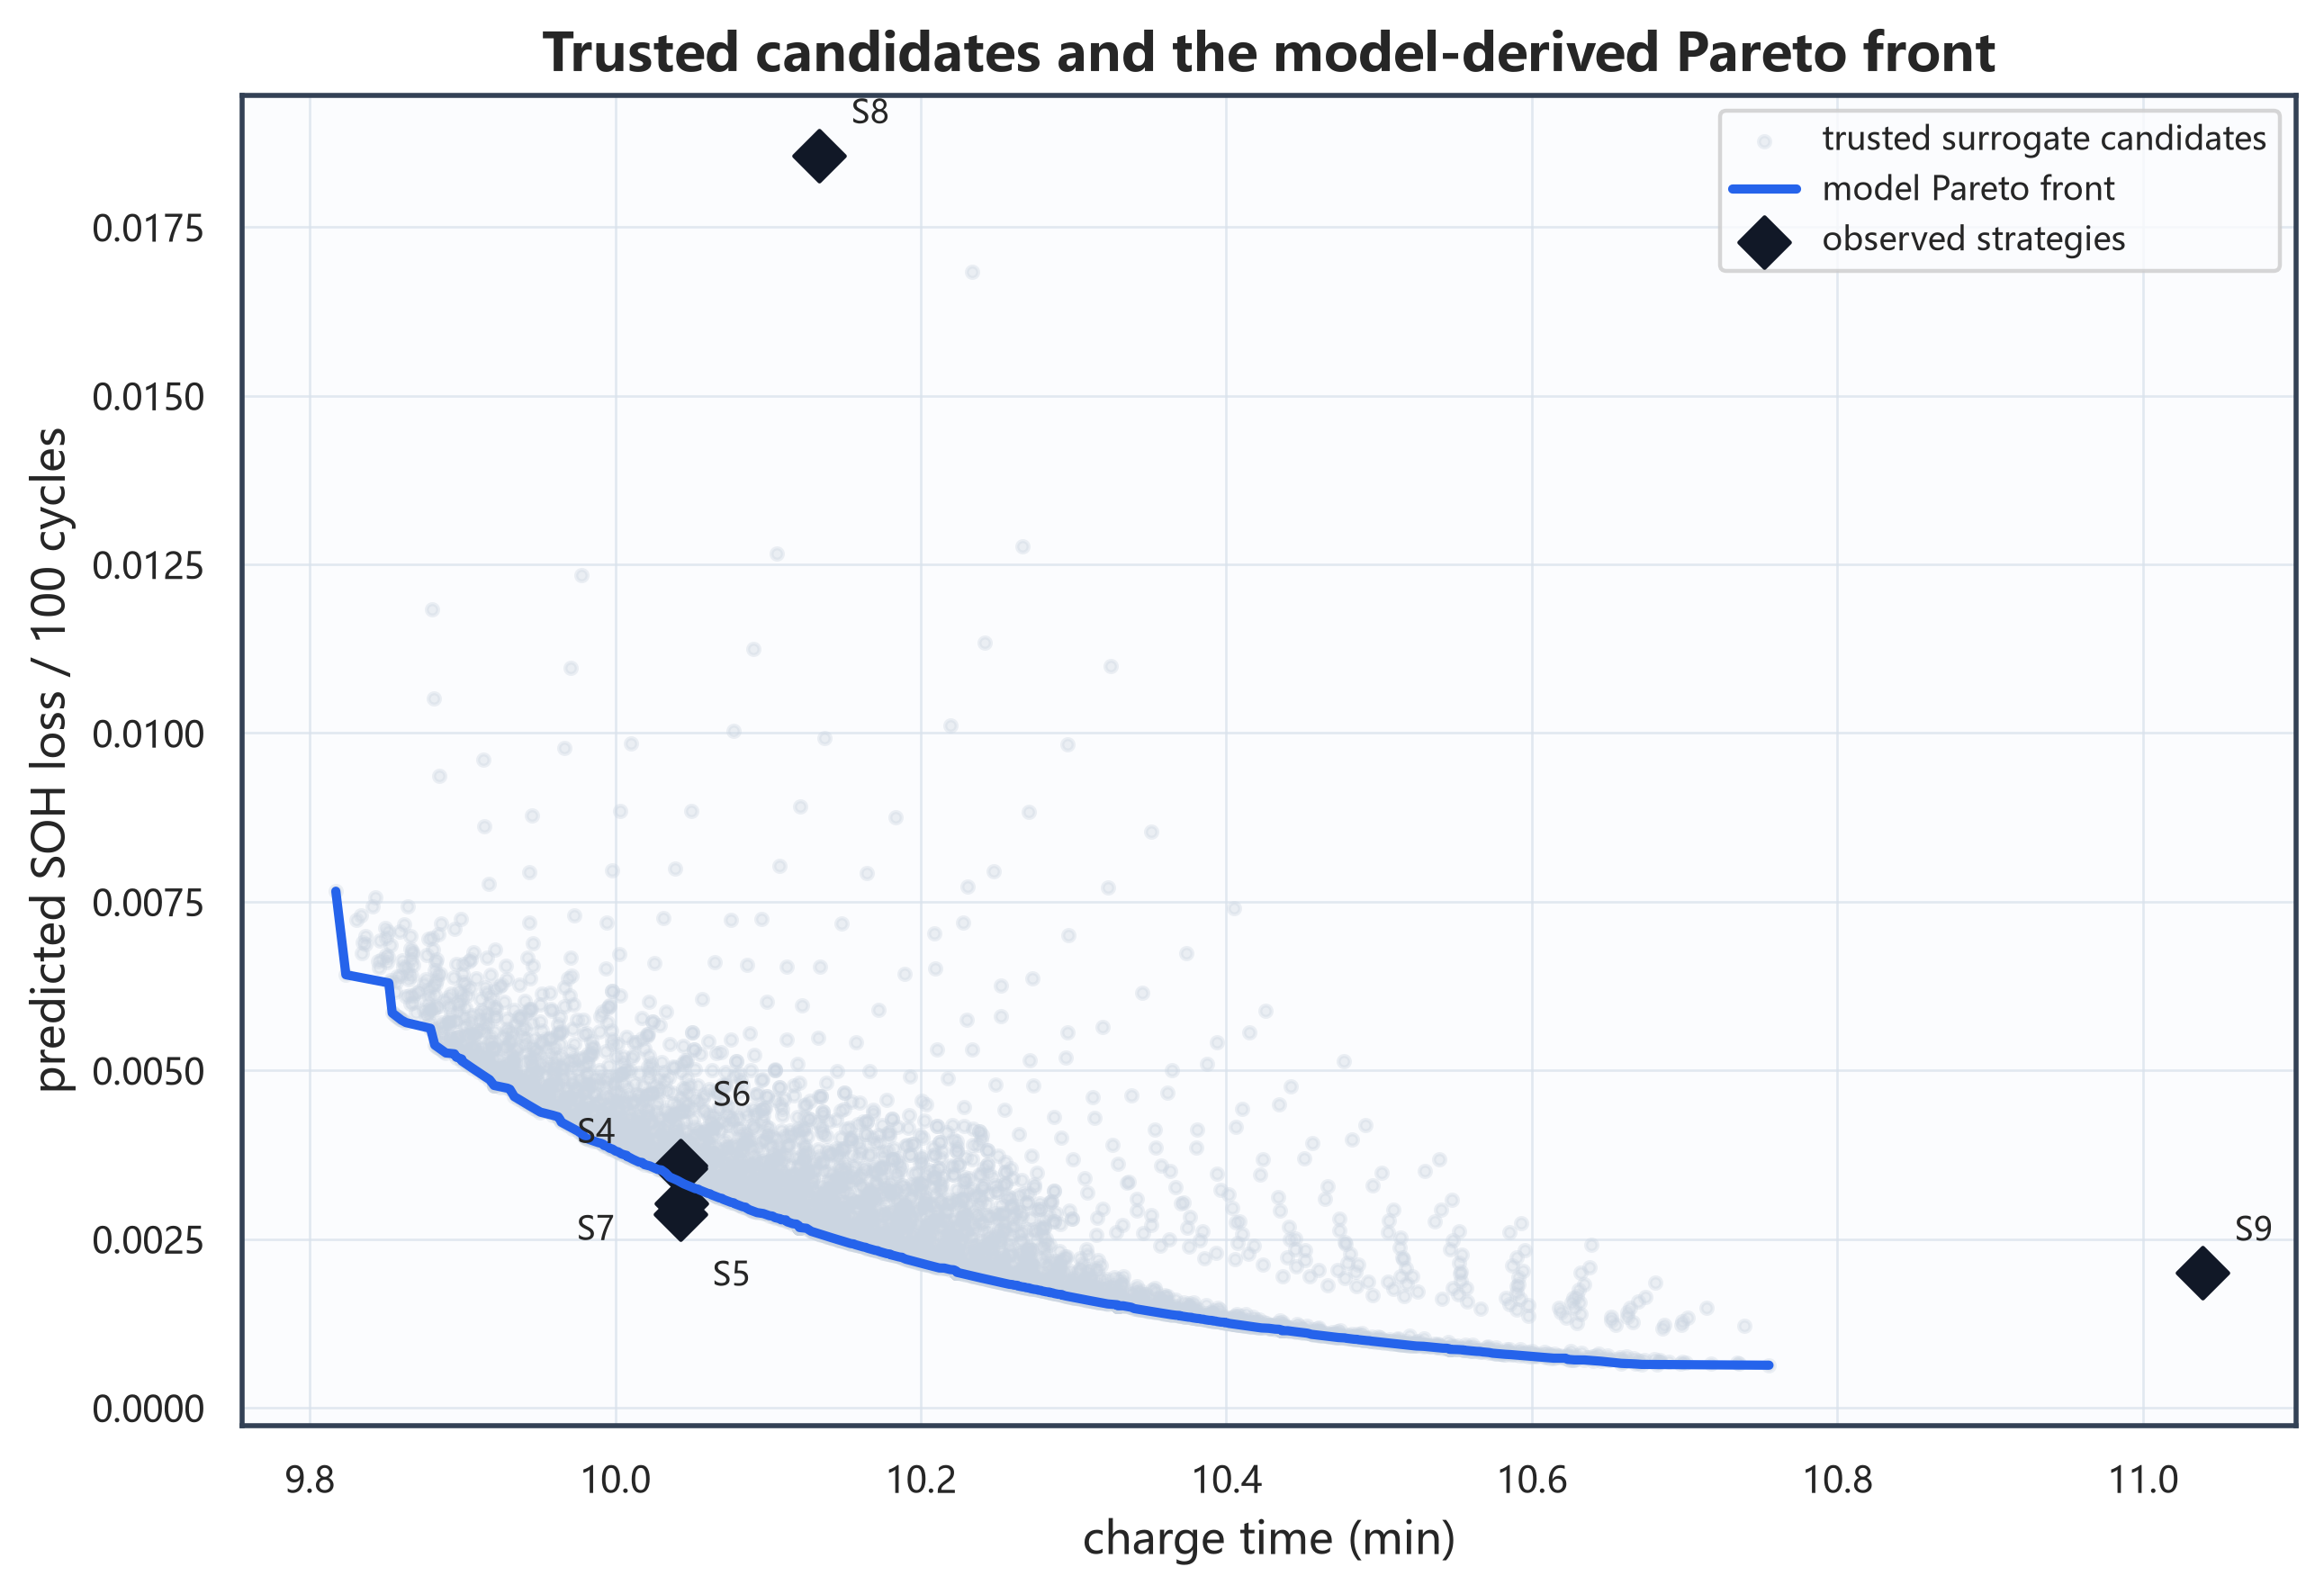
\includegraphics[width=0.9\textwidth]{q4_04_pareto_existing_candidates.png}
\caption{已有实验策略、可信域候选与 Pareto 前沿}
\label{fig:q4pareto}
\end{figure}

\begin{figure}[H]
\centering
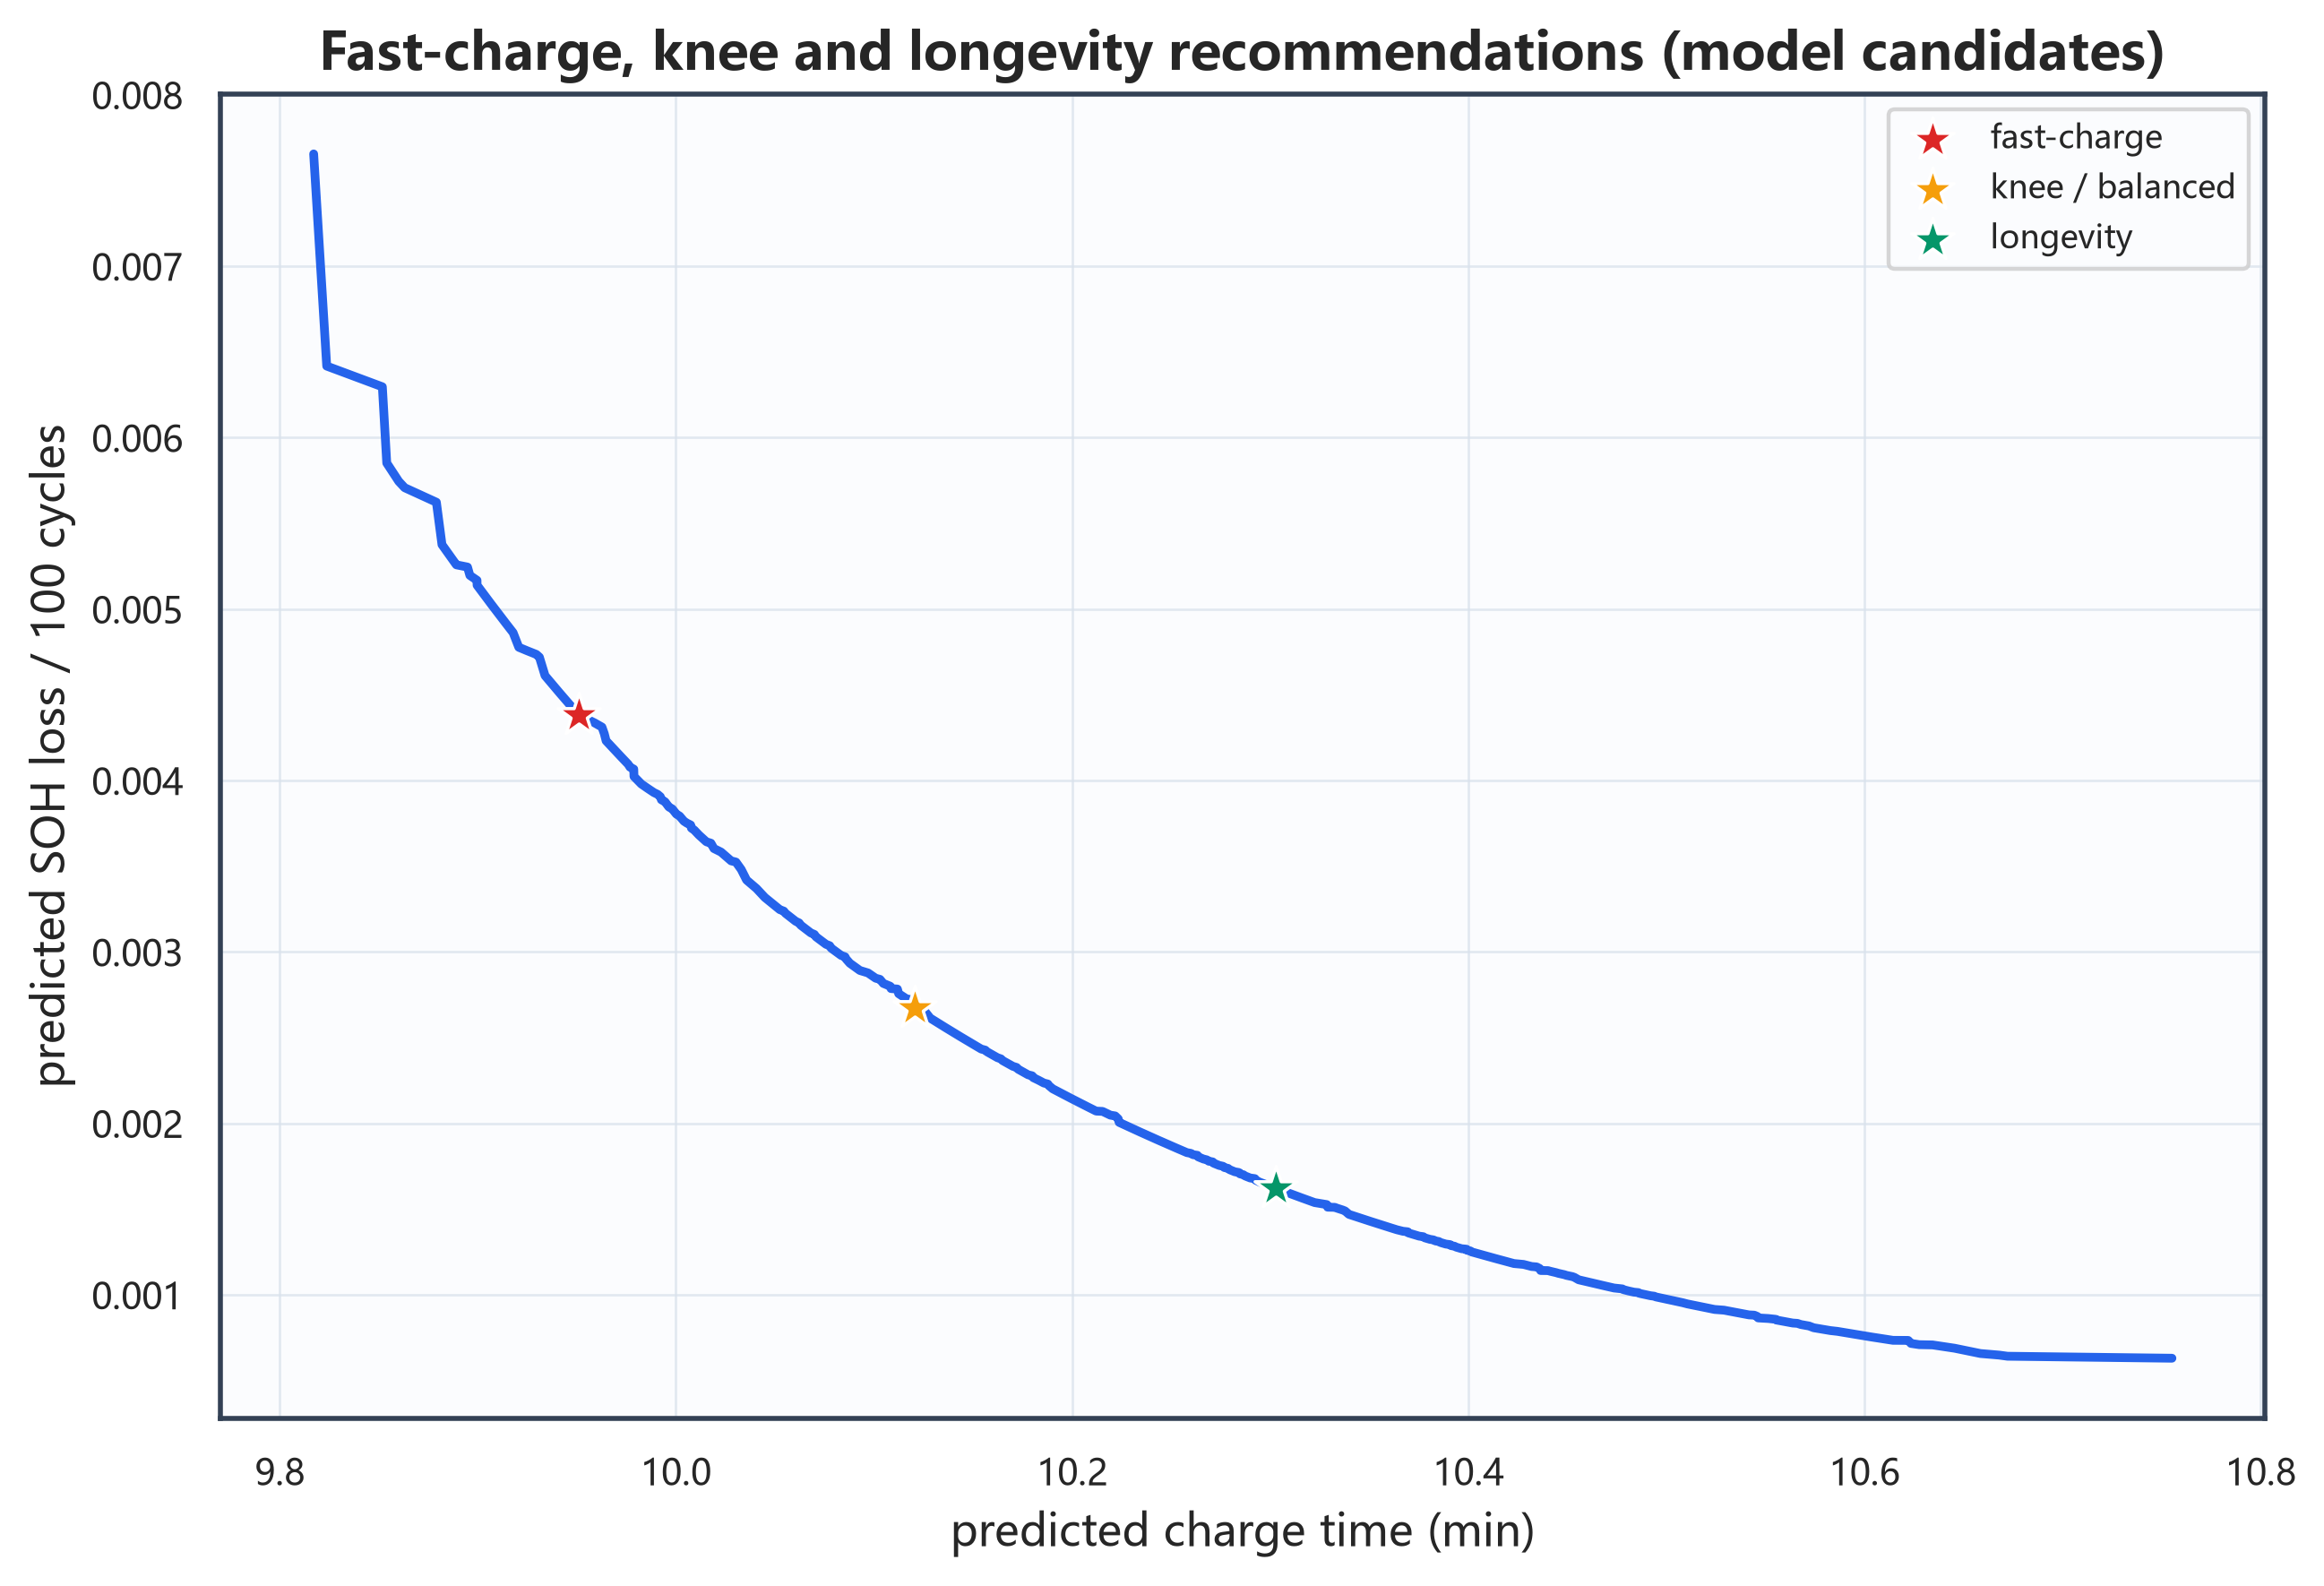
\includegraphics[width=0.88\textwidth]{q4_05_recommendations_on_pareto.png}
\caption{快充型、knee 折中型和寿命型代表点}
\label{fig:q4recommend}
\end{figure}

\subsection{推荐方案与风险解释}

\begin{table}[H]
\centering
\caption{可信域内三类模型推荐}
\resizebox{\textwidth}{!}{
\begin{tabular}{lcccccccc}
\toprule
类型 & $C_1$/C & $Q_1$/\% & $C_2$/C & 时间/min & SOH$_{200}$ & $D$/100次 & EOL/次 & 置信度 \\
\midrule
快充型 & 5.00 & 28 & 4.90 & 9.951 & 0.9927 & 0.00438 & 1340 & 低 \\
knee 折中型 & 4.85 & 55 & 4.85 & 10.121 & 0.9957 & 0.00267 & 1472 & 中等 \\
寿命型 & 4.75 & 60 & 4.80 & 10.303 & 0.9974 & 0.00162 & 1619 & 中等 \\
\bottomrule
\end{tabular}}
\end{table}

快充、knee、寿命型的预测时间 95\% 区间分别为 [9.10,10.80]、[9.27,10.97]、[9.45,11.15] min；条件性 EOL 区间分别为 [1250,1429]、[1359,1585]、[1442,1796] 次。从快充型移至 knee，代理预测增加 0.170 min（约 10.2 s），$D$ 下降 0.00171/100 次（约 39\%），EOL 增加约 133 次；再移至寿命型，增加 0.182 min，$D$ 再下降 0.00105/100 次，EOL 再增加约 147 次。该“少量时间换取较大退化下降”的弯折只用于候选排序，因为 0.439 min 的时间模型 RMSE 已大于相邻代表点的时间差。

对 $p$、退化响应、可信域、逐策略删除、dataset 范围及代理参数 bootstrap 的敏感性分析显示：快充型 $Q_1$ 可由约 28\% 漂移至 63\%，稳定性低；knee 与寿命侧反复落在 $C_1,C_2\approx4.8\sim4.9$ C、$Q_1\approx55\%\sim60\%$ 的邻域，故应推荐“区域”而不是精确单点。参数覆盖与优化点位置见图\ref{fig:q4coverage}。

\begin{figure}[H]
\centering
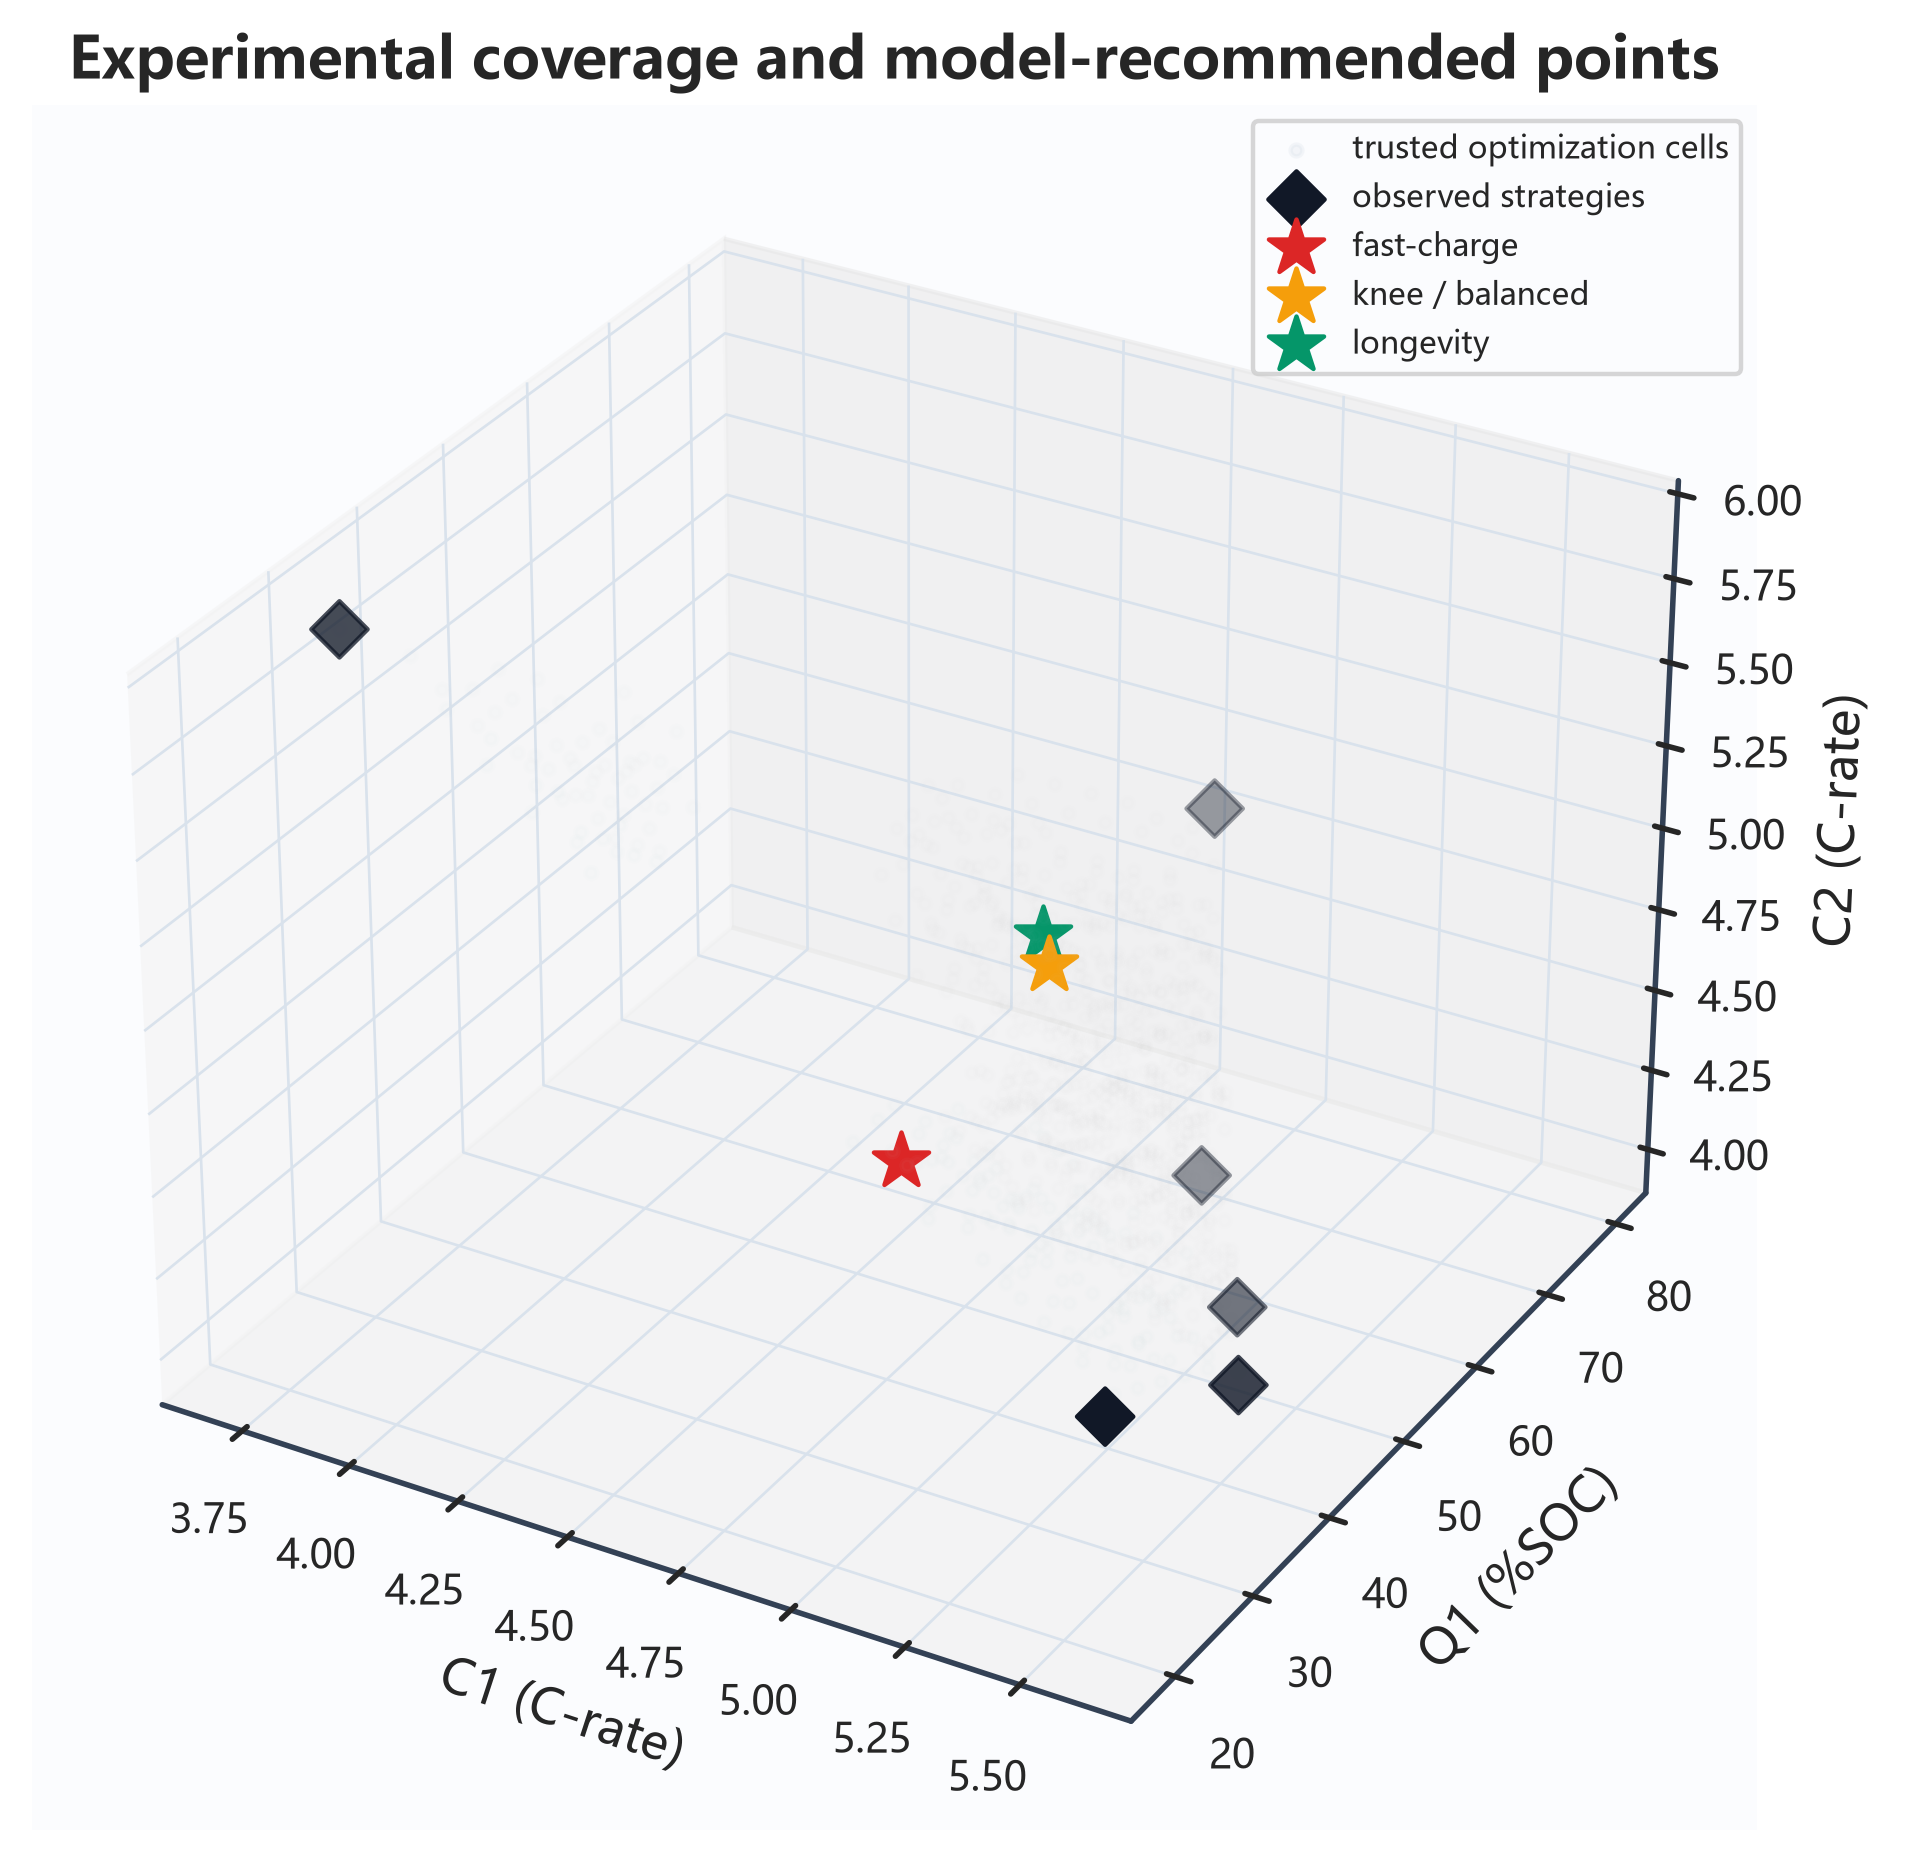
\includegraphics[width=0.88\textwidth]{q4_17_experimental_coverage.png}
\caption{实验参数覆盖、凸包边界与模型推荐位置}
\label{fig:q4coverage}
\end{figure}

与现有方案相比，S8 的实测 $D=0.01856$/100 次，是中高 SOC 高倍率的负面参照；S4--S7 约 10 min 且早期退化相对低，是可复现实验基线；S9 的 EOL 点估计较高但实测充电时间约 11.04 min，存在无法由三参数解释的批次/结构残差。因此，knee/寿命型只代表相对现有策略的预测改善趋势，推荐在该邻域新增实验后再决定工程采用。

\section{模型评价、局限与改进方向}\label{sec:evaluation}

本文的主要优点有三点。第一，清洗局部且可追溯，未用官方平滑列替代原始证据；时间截断和留一电池验证与真实使用场景一致。第二，问题一至四共享同一 SOH 和 EOL 口径，并以 SOH$_{200}$、早期斜率和 EOL 三类响应交叉核验，避免只靠长期外推得出参数结论。第三，多目标优化同时使用同批次限制、凸包和局部信任域，每个候选均带最近邻距离和不确定性，能显式暴露外推风险。

局限同样明确：训练策略仅 9 种，参数完整者 8 种，NEWSTRUCTURE 连续优化仅有 6 个设计点；strategy 与 batch 不完全可分离，S8 对应力--退化拟合影响较大；附件没有真实 EOL，因此任何寿命区间都未覆盖未知的长期机理变化；9 块测试电池的经验预测区间受小样本尾部估计限制；温度、内阻与充电时间可能同时受结构、环境和测量系统影响，不能直接解释为退化原因。

后续最有效的改进不是增加模型复杂度，而是在稳健优选区域安排验证实验：围绕 $C_1,C_2=4.7\sim5.0$ C、$Q_1=50\%\sim65\%$ 作小范围设计，并设置同批次重复电池；同时延长部分电池至真实 80\% SOH，以校准二次外推和模型结构误差。若获得更多独立策略点，可再比较分层贝叶斯模型或高斯过程，但仍应保持按电池、按策略的外层验证。

\section{结论}\label{sec:conclusion}

本文形成以下结论：
\begin{enumerate}
  \item 仅 3 个孤立物理异常需要局部修复。稳健 LOWESS 与 Theil--Sen 特征可在不扭曲总体趋势的情况下稳定表征早期退化。受约束二次模型在时间截断验证中兼顾短期误差、单调性和 EOL 稳定性；40 块训练电池条件性 EOL 中位数为 1348.7 次，但绝对寿命受模型结构限制。
  \item 充电策略对 SOH$_{200}$、50--200 次退化率和 EOL 的总体差异达到置换检验显著水平，S8 的早期退化最明显。较高 $C_2$ 和高 SOC 持续高倍率呈不利趋势，但该关系在控制 batch 后减弱，不能称为独立因果效应。
  \item 同策略群体模板与个体早期修正的自适应集成在严格留一电池伪测试中达到平均 MAE $2.77\times10^{-4}$、RMSE $3.61\times10^{-4}$，优于直接单电池外推。B2、B5、B25 偏离同策略群体较多；B16 的短期预测在当前模型内相对稳定，但其早期下降最快。
  \item 在 NEWSTRUCTURE 的凸包与局部信任域内，充电时间--退化前沿存在明显弯折。建议优先验证 $C_1,C_2\approx4.8\sim4.9$ C、$Q_1\approx55\%\sim60\%$ 的区域；knee 点 $(4.85\mathrm C,55\%,4.85\mathrm C)$ 是代表性实验候选，而不是已验证最优策略。
\end{enumerate}

\section*{AI 工具使用声明}

本参赛队在竞赛过程中使用了 AI 工具，主要用于题面信息整理、程序结构设计、代码调试、结果复核、图表生成与语言润色；所有数据处理口径、统计结论、模型选择和论文内容均需由参赛队逐项人工审查与核验，详细使用情况见支撑材料。

\begin{thebibliography}{99}
\bibitem{severson2019} Severson K A, Attia P M, Jin N, et al. Data-driven prediction of battery cycle life before capacity degradation[J]. Nature Energy, 2019, 4: 383--391.
\bibitem{attia2020} Attia P M, Grover A, Jin N, et al. Closed-loop optimization of fast-charging protocols for batteries with machine learning[J]. Nature, 2020, 578: 397--402.
\bibitem{cleveland1979} Cleveland W S. Robust locally weighted regression and smoothing scatterplots[J]. Journal of the American Statistical Association, 1979, 74(368): 829--836.
\bibitem{sen1968} Sen P K. Estimates of the regression coefficient based on Kendall's tau[J]. Journal of the American Statistical Association, 1968, 63(324): 1379--1389.
\bibitem{welch1951} Welch B L. On the comparison of several mean values: an alternative approach[J]. Biometrika, 1951, 38(3/4): 330--336.
\bibitem{kruskal1952} Kruskal W H, Wallis W A. Use of ranks in one-criterion variance analysis[J]. Journal of the American Statistical Association, 1952, 47(260): 583--621.
\bibitem{holm1979} Holm S. A simple sequentially rejective multiple test procedure[J]. Scandinavian Journal of Statistics, 1979, 6(2): 65--70.
\bibitem{efron1979} Efron B. Bootstrap methods: another look at the jackknife[J]. The Annals of Statistics, 1979, 7(1): 1--26.
\bibitem{hoerl1970} Hoerl A E, Kennard R W. Ridge regression: biased estimation for nonorthogonal problems[J]. Technometrics, 1970, 12(1): 55--67.
\bibitem{cliff1993} Cliff N. Dominance statistics: ordinal analyses to answer ordinal questions[J]. Psychological Bulletin, 1993, 114(3): 494--509.
\end{thebibliography}

\clearpage
\appendix
\section{支撑材料文件清单}

\begin{longtable}{p{0.26\textwidth}p{0.66\textwidth}}
\toprule
路径 & 内容 \\
\midrule
\endfirsthead
\toprule
路径 & 内容 \\
\midrule
\endhead
\nolinkurl{data/raw/} & 题目原始电池汇总表与循环数据，只读保留。 \\
\nolinkurl{data/processed/question1/} & 局部异常修复并重建稳健 SOH 后的循环级数据。 \\
\nolinkurl{outputs/question1/tables/} & 数据审计、早期特征、截断验证、候选模型、单电池及策略寿命表。 \\
\nolinkurl{outputs/question2/tables/} & 策略差异检验、效应量、共线性、回归、stress 与 batch 敏感性结果。 \\
\nolinkurl{outputs/question3/tables/} & 40 块训练电池伪测试、9 块测试电池逐循环预测、区间与 EOL。 \\
\nolinkurl{outputs/question4/tables/} & 时间/退化代理验证、可信域网格、Pareto 候选、推荐及鲁棒性分析。 \\
\nolinkurl{figures/question1--4/} & 全部候选图的 320 dpi PNG 与 SVG 矢量版本。 \\
\nolinkurl{docs/} & 题面口径、方法、结果说明及 AI 工具使用记录。 \\
\nolinkurl{src/}，\nolinkurl{scripts/} & 模块化源代码与四问可重复运行入口。 \\
\nolinkurl{tests/} & 数据完整性、泄漏边界和关键模型逻辑测试。 \\
\bottomrule
\end{longtable}

\section{复现方法}

在项目根目录执行：
\begin{lstlisting}[language=bash]
python -m venv .venv
.venv\Scripts\python.exe -m pip install -r requirements.txt
.venv\Scripts\python.exe -m pip install -e .
.venv\Scripts\python.exe scripts\run_question1.py --bootstrap-samples 300
.venv\Scripts\python.exe scripts\run_question2.py
.venv\Scripts\python.exe scripts\run_question3.py
.venv\Scripts\python.exe scripts\run_question4.py --bootstrap-samples 300
.venv\Scripts\python.exe -m pytest -q
\end{lstlisting}
所有随机过程使用固定种子；各问题的 \texttt{manifest.json} 记录生成文件清单。

\section{完整源程序}

\subsection{运行入口}
\lstinputlisting[caption={数据审计入口}]{../scripts/audit_data.py}
\lstinputlisting[caption={问题一运行入口}]{../scripts/run_question1.py}
\lstinputlisting[caption={问题二运行入口}]{../scripts/run_question2.py}
\lstinputlisting[caption={问题三运行入口}]{../scripts/run_question3.py}
\lstinputlisting[caption={问题四运行入口}]{../scripts/run_question4.py}

\subsection{公共数据、特征与问题一模块}
\lstinputlisting[caption={全局配置}]{../src/celianbei_dbatzrljy/config.py}
\lstinputlisting[caption={数据读取与稳健清洗}]{../src/celianbei_dbatzrljy/data.py}
\lstinputlisting[caption={早期退化特征}]{../src/celianbei_dbatzrljy/features.py}
\lstinputlisting[caption={退化候选模型与寿命估计}]{../src/celianbei_dbatzrljy/models.py}
\lstinputlisting[caption={策略汇总}]{../src/celianbei_dbatzrljy/summaries.py}
\lstinputlisting[caption={问题一绘图}]{../src/celianbei_dbatzrljy/plotting.py}
\lstinputlisting[caption={问题一流水线}]{../src/celianbei_dbatzrljy/pipeline.py}

\subsection{问题二模块}
\lstinputlisting[caption={问题二统计方法}]{../src/celianbei_dbatzrljy/question2_stats.py}
\lstinputlisting[caption={问题二绘图}]{../src/celianbei_dbatzrljy/question2_plotting.py}
\lstinputlisting[caption={问题二流水线}]{../src/celianbei_dbatzrljy/question2_pipeline.py}

\subsection{问题三模块}
\lstinputlisting[caption={问题三预测模型}]{../src/celianbei_dbatzrljy/question3_models.py}
\lstinputlisting[caption={问题三绘图}]{../src/celianbei_dbatzrljy/question3_plotting.py}
\lstinputlisting[caption={问题三流水线}]{../src/celianbei_dbatzrljy/question3_pipeline.py}

\subsection{问题四模块}
\lstinputlisting[caption={问题四代理与 Pareto 方法}]{../src/celianbei_dbatzrljy/question4_models.py}
\lstinputlisting[caption={问题四绘图}]{../src/celianbei_dbatzrljy/question4_plotting.py}
\lstinputlisting[caption={问题四流水线}]{../src/celianbei_dbatzrljy/question4_pipeline.py}

\end{document}
